%% abtex2-modelo-trabalho-academico.tex, v-1.7.1 laurocesar
%% Copyright 2012-2013 by abnTeX2 group at http://abntex2.googlecode.com/ 
%%
%% This work may be distributed and/or modified under the
%% conditions of the LaTeX Project Public License, either version 1.3
%% of this license or (at your option) any later version.
%% The latest version of this license is in
%%   http://www.latex-project.org/lppl.txt
%% and version 1.3 or later is part of all distributions of LaTeX
%% version 2005/12/01 or later.
%%
%% This work has the LPPL maintenance status `maintained'.
%% 
%% The Current Maintainer of this work is the abnTeX2 team, led
%% by Lauro César Araujo. Further information are available on 
%% http://abntex2.googlecode.com/
%%
%% This work consists of the files abntex2-modelo-trabalho-academico.tex,
%% abntex2-modelo-include-comandos and abntex2-modelo-references.bib
%%

% ------------------------------------------------------------------------
% ------------------------------------------------------------------------
% abnTeX2: Modelo de Trabalho Academico (tese de doutorado, dissertacao de
% mestrado e trabalhos monograficos em geral) em conformidade com 
% ABNT NBR 14724:2011: Informacao e documentacao - Trabalhos academicos -
% Apresentacao
% ------------------------------------------------------------------------
% ------------------------------------------------------------------------

\documentclass[
	% -- opções da classe memoir --
	12pt,				% tamanho da fonte
	openright,			% capítulos começam em pág ímpar (insere página vazia caso preciso)
	twoside,			% para impressão em verso e anverso. Oposto a oneside
	a4paper,			% tamanho do papel. 
	% -- opções da classe abntex2 --
	%chapter=TITLE,		% títulos de capítulos convertidos em letras maiúsculas
	%section=TITLE,		% títulos de seções convertidos em letras maiúsculas
	%subsection=TITLE,	% títulos de subseções convertidos em letras maiúsculas
	%subsubsection=TITLE,% títulos de subsubseções convertidos em letras maiúsculas
	% -- opções do pacote babel --
	english,			% idioma adicional para hifenização
	french,				% idioma adicional para hifenização
	spanish,			% idioma adicional para hifenização
	brazil,				% o último idioma é o principal do documento
	]{abntex2}


% ---
% PACOTES
% ---

% ---
% Pacotes fundamentais 
% ---
\usepackage{cmap}				% Mapear caracteres especiais no PDF
\usepackage{lmodern}			% Usa a fonte Latin Modern			
\usepackage[T1]{fontenc}		% Selecao de codigos de fonte.
\usepackage[utf8]{inputenc}		% Codificacao do documento (conversão automática dos acentos)
\usepackage{lastpage}			% Usado pela Ficha catalográfica
\usepackage{indentfirst}		% Indenta o primeiro parágrafo de cada seção.
\usepackage{color}				% Controle das cores
\usepackage{graphicx}			% Inclusão de gráficos
\usepackage{subfig}				% Possibilidade de colocar subfiguras

%Para colocar um caminho padrão de figuras
\graphicspath{{Imagens/}}
% ---
		
% ---
% Pacotes adicionais, usados apenas no âmbito do Modelo Canônico do abnteX2
% ---
\usepackage{lipsum}				% para geração de dummy text
% ---

% Pacotes adicionais, centraliza legendas de multiplas linhas
% ---
\usepackage{caption}				% para geração de dummy text
% ---

% Numeração por capítulos
%-----
\counterwithin{figure}{chapter}
\counterwithin{table}{chapter}
%-----

% Código fonte destacado no documento
%-------
\usepackage{listings}
\usepackage[newfloat]{minted}
\usepackage{mdframed}
\usepackage{xcolor}
\definecolor{bg}{rgb}{0.95,0.95,0.95}
\usepackage{float}

%questões sobre legendas e listas
\renewcommand{\lstlistingname}{Código}% Listing -> Algorithm
\renewcommand{\lstlistlistingname}{Lista de \lstlistingname s}% List of Listings -> List of Algorithms
%-------

%-----
% Estilo de tabela
%-----
\usepackage{booktabs}
\usepackage{multirow}
\usepackage{array, makecell}
\usepackage{setspace}
\usepackage{cellspace}
\usepackage{diagbox}
\setlength\cellspacetoplimit{5pt}
\setlength\cellspacebottomlimit{5pt}

%-----
% Reduzir espaço entre figura e texto
%------
%\usepackage{etoolbox}
%\BeforeBeginEnvironment{figure}{\vskip-2ex}
%\AfterEndEnvironment{figure}{\vskip-1ex}

%-------
% Comandos personalizados
%-------
\newcommand{\duvida}[1]{\textcolor{red}{#1}}


% ---
% Pacotes de citações
% ---
%\usepackage[brazilian,hyperpageref]{backref}	 % Paginas com as citações na bibl
%\usepackage[alf,abnt-etal-list=0,abnt-etal-cite=3]{abntex2cite}	% Citações padrão ABNT

\usepackage[style=abnt,backref=true,backend=biber,citecounter=true]{biblatex}
\addbibresource{abntex2-modelo-references.bib}

%Texto padrão antes do número das páginas
\DefineBibliographyStrings{brazil}{%
	backrefpage = {Citado na página},% originally "cited on page"
	backrefpages = {Citado \arabic{citecounter} vezes nas páginas},% originally "cited on pages"
}

% --- 
% CONFIGURAÇÕES DE PACOTES
% --- 

% ---
% Configurações do pacote backref
% Usado sem a opção hyperpageref de backref
%\renewcommand{\backrefpagesname}{Citado na(s) página(s):~}
%% Texto padrão antes do número das páginas
%\renewcommand{\backref}{}
%% Define os textos da citação
%\renewcommand*{\backrefalt}[4]{
%	\ifcase #1 %
%		Nenhuma citação no texto.%
%	\or
%		Citado na página #2.%
%	\else
%		Citado #1 vezes nas páginas #2.%
%	\fi}%
%% ---


% ---
% Informações de dados para CAPA e FOLHA DE ROSTO
% ---
\titulo{Desenvolvimento de uma Plataforma Embarcada para Monitoramento e Operação de um Trocador de Calor}
\autor{Felipe Rodrigues Pereira Fonseca}
\local{Belo Horizonte}
\data{Novembro de 2017}
\orientador{Lúcio Fábio Dias Passos, DEQ/UFMG}
%\coorientador{Equipe \abnTeX}
\instituicao{%
  Universidade Federal de Minas Gerais
  \par
  Escola de Engenharia
  \par
  Curso de Graduação em Engenharia de Controle e Automação}
\tipotrabalho{Monografia de Projeto Final de Curso}
% O preambulo deve conter o tipo do trabalho, o objetivo, 
% o nome da instituição e a área de concentração 
\preambulo{Monografia submetida à banca examinadora designada pelo Colegiado Didático do Curso de Graduação em Engenharia de Controle e Automação da Universidade Federal de Minas Gerais,como parte dos requisitos para aprovação na disciplina Projeto Final de Curso II.}
% ---


% ---
% Configurações de aparência do PDF final

% alterando o aspecto da cor azul
\definecolor{blue}{RGB}{41,5,195}

% informações do PDF
\makeatletter
\hypersetup{
     	%pagebackref=true,
		pdftitle={\@title}, 
		pdfauthor={\@author},
    	pdfsubject={\imprimirpreambulo},
	    pdfcreator={LaTeX with abnTeX2},
		pdfkeywords={abnt}{latex}{abntex}{abntex2}{trabalho acadêmico}, 
		colorlinks=true,       		% false: boxed links; true: colored links
    	linkcolor=blue,          	% color of internal links
    	citecolor=blue,        		% color of links to bibliography
    	filecolor=magenta,      		% color of file links
		urlcolor=blue,
		bookmarksdepth=4
}
\makeatother
% --- 

% --- 
% Espaçamentos entre linhas e parágrafos 
% --- 

% O tamanho do parágrafo é dado por:
\setlength{\parindent}{1.3cm}

% Controle do espaçamento entre um parágrafo e outro:
\setlength{\parskip}{0.2cm}  % tente também \onelineskip

% ---
% compila o indice
% ---
\makeindex
% ---

% ----
% Início do documento
% ----
\begin{document}

% Retira espaço extra obsoleto entre as frases.
\frenchspacing 

% ----------------------------------------------------------
% ELEMENTOS PRÉ-TEXTUAIS
% ----------------------------------------------------------
% \pretextual

% ---
% Capa
% ---
\imprimircapa
% ---

% ---
% Folha de rosto
% (o * indica que haverá a ficha bibliográfica)
% ---
\imprimirfolhaderosto*
% ---

% ---
% Inserir a ficha bibliografica
% ---

% Isto é um exemplo de Ficha Catalográfica, ou ``Dados internacionais de
% catalogação-na-publicação''. Você pode utilizar este modelo como referência. 
% Porém, provavelmente a biblioteca da sua universidade lhe fornecerá um PDF
% com a ficha catalográfica definitiva após a defesa do trabalho. Quando estiver
% com o documento, salve-o como PDF no diretório do seu projeto e substitua todo
% o conteúdo de implementação deste arquivo pelo comando abaixo:
%
% \begin{fichacatalografica}
%     \includepdf{fig_ficha_catalografica.pdf}
% \end{fichacatalografica}
\begin{fichacatalografica}
	\vspace*{\fill}					% Posição vertical
	\hrule							% Linha horizontal
	\begin{center}					% Minipage Centralizado
	\begin{minipage}[c]{12.5cm}		% Largura
	
	\imprimirautor
	
	\hspace{0.5cm} \imprimirtitulo  / \imprimirautor. --
	\imprimirlocal, \imprimirdata-
	
	\hspace{0.5cm} \pageref{LastPage} p. : il. (algumas color.) ; 30 cm.\\
	
	\hspace{0.5cm} \imprimirorientadorRotulo~\imprimirorientador\\
	
	\hspace{0.5cm}
	\parbox[t]{\textwidth}{\imprimirtipotrabalho~--~\imprimirinstituicao,
	\imprimirdata.}\\
	
	\hspace{0.5cm}
		1. Palavra-chave1.
		2. Palavra-chave2.
		I. Orientador.
		II. Universidade xxx.
		III. Faculdade de xxx.
		IV. Título\\ 			
	
	\hspace{8.75cm} CDU 02:141:005.7\\
	
	\end{minipage}
	\end{center}
	\hrule
\end{fichacatalografica}
% ---

% ---
% Inserir errata
% ---
%\begin{errata}
%Elemento opcional da \citeonline[4.2.1.2]{NBR14724:2011}. Exemplo:
%
%\vspace{\onelineskip}
%
%FERRIGNO, C. R. A. \textbf{Tratamento de neoplasias ósseas apendiculares com
%reimplantação de enxerto ósseo autólogo autoclavado associado ao plasma
%rico em plaquetas}: estudo crítico na cirurgia de preservação de membro em
%cães. 2011. 128 f. Tese (Livre-Docência) - Faculdade de Medicina Veterinária e
%Zootecnia, Universidade de São Paulo, São Paulo, 2011.
%
%\begin{table}[htb]
%\center
%\footnotesize
%\begin{tabular}{|p{1.4cm}|p{1cm}|p{3cm}|p{3cm}|}
%  \hline
%   \textbf{Folha} & \textbf{Linha}  & \textbf{Onde se lê}  & \textbf{Leia-se}  \\
%    \hline
%    1 & 10 & auto-conclavo & autoconclavo\\
%   \hline
%\end{tabular}
%\end{table}
%
%\end{errata}
% ---

% ---
% Inserir folha de aprovação
% ---

% Isto é um exemplo de Folha de aprovação, elemento obrigatório da NBR
% 14724/2011 (seção 4.2.1.3). Você pode utilizar este modelo até a aprovação
% do trabalho. Após isso, substitua todo o conteúdo deste arquivo por uma
% imagem da página assinada pela banca com o comando abaixo:
%
% \includepdf{folhadeaprovacao_final.pdf}
%
\begin{folhadeaprovacao}

  \begin{center}
    {\ABNTEXchapterfont\large\imprimirautor}

    \vspace*{\fill}\vspace*{\fill}
    {\ABNTEXchapterfont\bfseries\Large\imprimirtitulo}
    \vspace*{\fill}
    
    \hspace{.45\textwidth}
    \begin{minipage}{.5\textwidth}
        \imprimirpreambulo
    \end{minipage}%
    \vspace*{\fill}
   \end{center}
    
   Trabalho aprovado. \imprimirlocal, 24 de novembro de 2012:

   \assinatura{\textbf{\imprimirorientador} \\ Orientador} 
   \assinatura{\textbf{Professor} \\ Convidado 1}
   \assinatura{\textbf{Professor} \\ Convidado 2}
   %\assinatura{\textbf{Professor} \\ Convidado 3}
   %\assinatura{\textbf{Professor} \\ Convidado 4}
      
   \begin{center}
    \vspace*{0.5cm}
    {\large\imprimirlocal}
    \par
    {\large\imprimirdata}
    \vspace*{1cm}
  \end{center}
  
\end{folhadeaprovacao}
% ---

% ---
% Dedicatória
% ---
\begin{dedicatoria}
   \vspace*{\fill}
   \centering
   \noindent
   \textit{ Este trabalho é dedicado às crianças adultas que,\\
   quando pequenas, sonharam em se tornar cientistas.} \vspace*{\fill}
\end{dedicatoria}
% ---

% ---
% Agradecimentos
% ---
\begin{agradecimentos}
Os agradecimentos principais são direcionados à Gerald Weber, Miguel Frasson,
Leslie H. Watter, Bruno Parente Lima, Flávio de Vasconcellos Corrêa, Otavio Real
Salvador, Renato Machnievscz\footnote{Os nomes dos integrantes do primeiro
projeto abn\TeX\ foram extraídos de
\url{http://codigolivre.org.br/projects/abntex/}} e todos aqueles que
contribuíram para que a produção de trabalhos acadêmicos conforme
as normas ABNT com \LaTeX\ fosse possível.

Agradecimentos especiais são direcionados ao Centro de Pesquisa em Arquitetura
da Informação\footnote{\url{http://www.cpai.unb.br/}} da Universidade de
Brasília (CPAI), ao grupo de usuários
\emph{latex-br}\footnote{\url{http://groups.google.com/group/latex-br}} e aos
novos voluntários do grupo
\emph{\abnTeX}\footnote{\url{http://groups.google.com/group/abntex2} e
\url{http://abntex2.googlecode.com/}}~que contribuíram e que ainda
contribuirão para a evolução do \abnTeX.

\end{agradecimentos}
% ---

% ---
% Epígrafe
% ---
\begin{epigrafe}
    \vspace*{\fill}
	\begin{flushright}
		\textit{``Não vos amoldeis às estruturas deste mundo, \\
		mas transformai-vos pela renovação da mente, \\
		a fim de distinguir qual é a vontade de Deus: \\
		o que é bom, o que Lhe é agradável, o que é perfeito.\\
		(Bíblia Sagrada, Romanos 12, 2)}
	\end{flushright}
\end{epigrafe}
% ---

% ---
% RESUMOS
% ---

% resumo em português
\begin{resumo}
 Resumo

 \vspace{\onelineskip}
    
 \noindent
 \textbf{Palavras-chaves}: latex. abntex. editoração de texto.
\end{resumo}

% resumo em inglês
\begin{resumo}[Abstract]
 \begin{otherlanguage*}{english}
   This is the english abstract.

   \vspace{\onelineskip}
 
   \noindent 
   \textbf{Key-words}: latex. abntex. text editoration.
 \end{otherlanguage*}
\end{resumo}

% resumo em francês 
%\begin{resumo}[Résumé]
% \begin{otherlanguage*}{french}
%    Il s'agit d'un résumé en français.
% 
%   \vspace{\onelineskip}
% 
%   \noindent
%   \textbf{Mots-clés}: latex. abntex. publication de textes.
% \end{otherlanguage*}
%\end{resumo}

% resumo em espanhol
%\begin{resumo}[Resumen]
% \begin{otherlanguage*}{spanish}
%   Este es el resumen en español.
%  
%   \vspace{\onelineskip}
% 
%   \noindent
%   \textbf{Palabras clave}: latex. abntex. publicación de textos.
% \end{otherlanguage*}
%\end{resumo}
% ---

% ---
% inserir lista de ilustrações
% ---
\pdfbookmark[0]{\listfigurename}{lof}
\listoffigures*
\cleardoublepage
% ---

% ---
% inserir lista de tabelas
% ---
\pdfbookmark[0]{\listtablename}{lot}
\listoftables*
\cleardoublepage
% ---

% ---
% inserir lista de abreviaturas e siglas
% ---
\begin{siglas}
  \item[Fig.] Area of the $i^{th}$ component
  \item[456] Isto é um número
  \item[123] Isto é outro número
  \item[lauro cesar] este é o meu nome
\end{siglas}
% ---

% ---
% inserir lista de símbolos
% ---
\begin{simbolos}
  \item[$ \Gamma $] Letra grega Gama
  \item[$ \Lambda $] Lambda
  \item[$ \zeta $] Letra grega minúscula zeta
  \item[$ \in $] Pertence
\end{simbolos}
% ---

%-----
% inserir lista de códigos
%-----
\pdfbookmark[0]{\lstlistlistingname}{lot}
\lstlistoflistings
\cleardoublepage


% ---
% inserir o sumario
% ---
\pdfbookmark[0]{\contentsname}{toc}
\tableofcontents*
\cleardoublepage
% ---



% ----------------------------------------------------------
% ELEMENTOS TEXTUAIS
% ----------------------------------------------------------
\textual

%comando para setar a introdução como página 1
% FORA DA NORMA!!!
\setcounter{page}{1}

% ----------------------------------------------------------
% Introdução
% ----------------------------------------------------------
\chapter{Introdução}
	%\addcontentsline{toc}{chapter}{Introdução}
	\chapterprecis{Este capítulo apresenta a motivação e justificativa para a realização deste projeto e o local de desenvolvimento, bem como descreve brevemente a estrutura da monografia}
	\section{Motivação e Justificativa}

	Um trocador de calor pode ser definido como um dispositivo em que ocorre uma transferência de calor entre duas substâncias que estejam em temperaturas distintas. Geralmente, as substâncias envolvidas são fluidos. Os trocadores de calor podem ser classificados com relação a diversos critérios, como por exemplo o modo de troca de calor, tipo de construção, entre outros. \cite{kreith2011}
	
	Indústrias dos mais variados setores utilizam trocadores de calores para diversas funcionalidades, tais como:
	
	\begin{itemize}
		\item 
		Recuperar energia térmica gerada em algum processo, com o intuito de reduzir o consumo de energia da planta;
		\item 
		Transportar produtos em temperaturas predeterminadas.
	\end{itemize}

	Portanto, é de suma importância a utilização de um sistema de controle eficiente em plantas que contém trocadores de calor. Plantas como essa devem ser capazes de atender referências de temperatura bem como rejeitar de possíveis pertubações que podem ocorrer durante o funcionamento do processo. \cite{novazzi2007}. Além disso, soluções que permitem o monitoramento e operação remota das plantas são relevantes para o processo, uma vez que trocadores de calor podem estar instalados em ambientes de difícil acesso ou operando em altas temperaturas. A operação remota de plantas industriais traz outros benefícios como \cite{babau2009}:
	\begin{itemize}
		\item 
		Interface mais amigável de operação, que contribui para uma atuação mais rápida e assertiva;
		\item 
		Melhor acessibilidade aos dados coletados, o que permite a equipe de engenharia e de gestão analisar e e propor melhorias na operação.
	\end{itemize}

	Diferentes arquiteturas de sistema de supervisão (monitoramento e operação) e controle podem ser aplicadas em plantas industriais. Encontram-se plantas utilizando a tradicional topologia formada por PLC e um computador (PC) executando alguma ferramenta SCADA \footnote{\url{https://www.wonderware.com/hmi-scada/what-is-scada/}}, bem como é possível verificar a utilização de sistemas embarcados.\footnote{\url{http://files.comunidades.net/mutcom/ARTIGO_SIST_EMB.pdf}} A escolha entre uma ou outra arquitetura depende de uma série de fatores, como: funcionalidades disponibilizadas por cada ferramenta, custo, domínio do desenvolvedor para utilizar determinados softwares, entre outros.
	
	Um sistema embarcado pode ser definido como um sistema projetado para realizar tarefas específicas e geralmente fazem parte de uma aplicação maior, operando em tempo real e sem intervenção do usuário \cite{baskiyar2005}.  Devido ao avanço da tecnologia e o aumento do poder de processamento dos hardwares, os sistemas embarcados podem realizar cada vez mais tarefas, ou seja, disponibilizar mais funcionalidades aos usuários \cite{luiz2011}. Este fenômeno também ocorre para os softwares SCADA, que estão cada vez mais poderosos e oferecem cada vez mais recursos \cite{david2017}. Porém, quanto maior é a variabilidade de opções de projeto disponível, maior é a dificuldade de se alcançar uma padronização no desenvolvimento e, principalmente, uma padronização da comunicação entre os componentes, pois muitos sistemas ainda se comunicam em protocolo proprietário.
	
	\textcolor{red}{Colocar nesse parágrfo informações sobre a evolução na utilização de sistemas Web no controle de processo, abordando a necessidade crescente de comunicação de vários sistemas.}
	
	Este trabalho apresenta o desenvolvimento de um sistema de baixo custo para monitoramento e operação via Web de um trocador de calor localizado em um dos laboratórios do departamento da engenharia química da UFMG. Para isso, foram utilizados protocolos de comunicação e ferramentas de código aberto, para possibilitar futura integração de outros sistemas e/ou funcionalidades.
	
	O tema é relevante pois, a implementação proposta permite aos alunos que realizem as práticas no laboratório forma mais adequada, de forma que os esforços estejam concentrados na análise dos experimentos e identificação dos fenômenos, e não na coleta de dados e regulação da planta nos pontos de operação. Essa implementação também permite aos alunos de Engenharia de Controle e Automação estudar modelagem de sistemas e projeto de controladores. Por fim, a solução proposta também proporciona os alunos o contato com tecnologias emergentes e que podem ser utilizadas largamente nas indústrias.  
	
		
	
\section{Objetivos}
	De acordo com as informações expostas acima, este Projeto Final de Curso (PFC) possui o seguinte objetivo geral:
	
	\begin{itemize}
		\item 
		Propor e testar uma solução baseada em sistemas embarcados para monitoramento e operação remota de um trocador de calor.
	\end{itemize}
	
	Além do objetivo geral, o projeto possui também os seguintes objetivos específicos:
	
	\begin{itemize}
		\item 
		Comparar a solução embarcada com um software de prateleira tradicional;
		\item 
		Proporcionar uma base de conhecimento para implementações de sistemas semelhantes para outras plantas do laboratório;
		\item 
		Possibilitar a inserção de mais funcionalidades ao sistema, como por exemplo um algoritmo de autovalidação. da planta;
	\end{itemize}
	

\section{Local de Realização}
	O projeto foi desenvolvido no Laboratório de Operações e Processos Industriais, um dos laboratórios que pertencem ao Departamento de Engenharia Química (DEQ) da UFMG. Estes laboratórios são utilizados para fins didáticos e de pequisa.

\section{Estrutura da Monografia}
	O trabalho está dividido em 6 capítulos. O presente capítulo apresentou a motivação e os objetivos do trabalho. O capítulo 2 .... 


% ----------------------------------------------------------
% PARTE - preparação da pesquisa
% ----------------------------------------------------------
%\part{Preparação da pesquisa}

% ----------------------------------------------------------
% Capitulo com exemplos de comandos inseridos de arquivo externo 
% ----------------------------------------------------------

%\include{abntex2-modelo-include-comandos}

% ----------------------------------------------------------
% Parte de revisãod e literatura
% ----------------------------------------------------------
%\part{Revisão de Literatura}

% ---
% Capitulo de revisão de literatura
% ---
\chapter{Revisão Bibliográfica}
	\chapterprecis{Teste, teste}
	
	\section{Laboratório de Operações Unitárias - Contextualização}
		O Laboratório de Operações Unitárias (LOU-DQ) é um dos diversos laboratórios para fins de ensino e pesquisa pertencentes ao Departamento de Engenharia Química da UFMG (DEQ). Ainda existem outros laboratórios vinculados ao departamento cuja finalidade é prestar serviços às comunidades interna e externa à UFMG \footnote{\url{http://www.deq.ufmg.br/departamento/infraestrutura}}.
		
		O LOU possui quatro plantas didáticas: um sistema de trocador de calor, uma planta que implementa um processo de sedimentação, uma planta piloto de um hidrociclone e uma planta que implementa um processo de secagem.
		
		%explicar aqui agora sobre a planta de trocador existente
		O trocador de calor existente no laboratório, cuja imagem pode ser vista na \autoref{fig:lab}, é do tipo tubular. Este sistema, que é fabricado e fornecido pela Universidade de Santa Cecília\footnote{\url{http://cursos.unisanta.br/quimica/laborato/index.html}}, foi adquirido pela UFMG em 2002\footnote{Item 35 do catálogo disponível em: \url{http://cursos.unisanta.br/quimica/laborato/LOU-2016.pdf}}. Originalmente, a planta possui um botão para ligar e desligar bomba e aquecedor simultaneamente, bem como conta com 4 sensores de temperatura, cujos valores são exibidos e display LCDs. A medição de vazão de água quente era inferida através da utilização de uma Calha Parshall\footnote{Funcionamento da Calha Parshall: \url{http://www.dec.ufcg.edu.br/saneamento/PARSHALL.html}}, e a medição de água fria, através da indicação de um rotâmetro\footnote{\url{http://www.sensorsmag.com/components/basics-rotameters}}
		
		\begin{figure}[!htb]
			\centering
			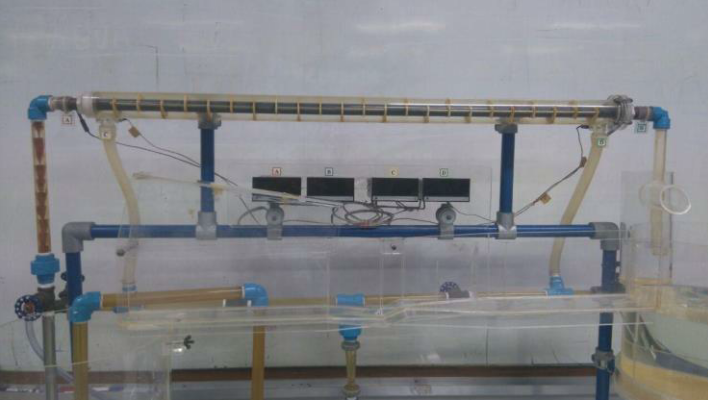
\includegraphics[scale=0.7]{lab}  %pode alterar o tamanho
			\caption{Trocador de Calor presente no LOU.}
			\label{fig:lab}
		\end{figure}

			
		Em 2016, um projeto de modernização desta planta foi iniciado por \cite{luiz2016}.  O projeto consistiu na implementação de um sistema embarcado para operação local e controle da planta. Para alcançar o objetivo, foram feitos os seguintes passos:
		\begin{itemize}
			\item 
			Instalação de quatro novos sensores de temperatura, dois novos sensores de vazão, tornando possível a medição digital das vazões; 2 relés, para o controle do acionamento dos atuadores e um inversor de frequência para controlar a rotação da bomba;
			\item 
			Instalação de um Arduino Due \footnote{\url{https://store.arduino.cc/usa/arduino-due}} para fazer a interface com sensores e atuadores, processar os algoritmos de controle, e exibir os dados em um display LCD. O programa criado no Arduino possibilita a operação em modo automático e manual;
			\item 
			Construção e instalação de um painel para operar e visualizar os dados da planta. Através desse painel é possível selecionar o modo de funcionamento da planta (manual ou automático). Em modo manual, é possível ligar e desligar bomba e aquecedor, bem como controlar a velocidade da bomba e potência do aquecedor. O display LCD permite exibir várias informações como por exemplo valores das temperaturas e vazões, bem como a sintonia dos controladores. Essas informações não conseguem ser expostas ao mesmo tempo para o usuário, portanto um sistema de navegação foi implementado no Arduino. O esboço do painel elaborado é mostrado na \autoref{fig:painel}.
		\end{itemize}
			
			\begin{figure}[!htb]	
				%\centering
				\captionsetup{justification=centering}
				\begin{center}
					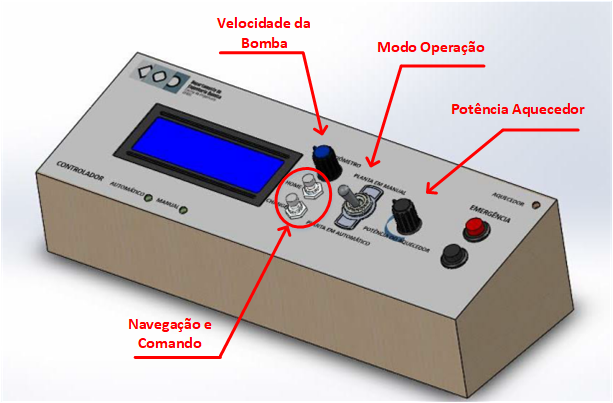
\includegraphics[scale=0.6]{painel}  %pode alterar o tamanho
					\caption[Painel instalado na planta de trocador de calor]{\label{fig:painel}Painel instalado na planta de trocador de calor. \\Adaptado de \cite{luiz2016}}
				\end{center}		
			\end{figure}
		
			A Arquitetura do sistema finalizado é exibida na \autoref{fig:arq_atual}. Destaca-se o fato que não foi possível integrar o controle da potência do aquecedor no Arduino, sendo enviado diretamente do painel. Apesar de previsto no projeto, nenhum algoritmo para controle em malha fechada foi programado.
		
			\begin{figure}[!htb]	
				%\centering
				\captionsetup{justification=centering}
				\begin{center}
					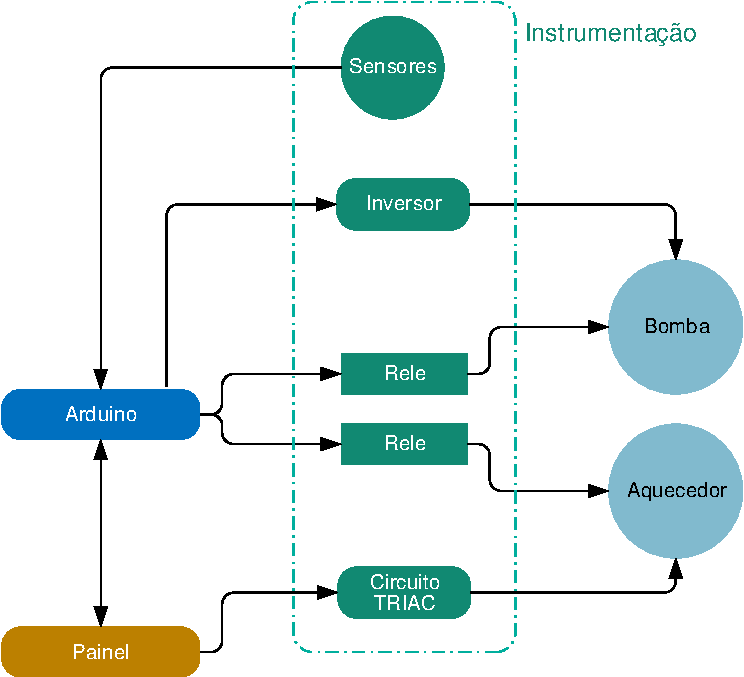
\includegraphics[scale=0.8]{arq_atual}  %pode alterar o tamanho
					\caption[Arquitetura do sistema instalado]{\label{fig:arq_atual}Arquitetura do sistema instalado}
				\end{center}		
			\end{figure}
		
	
	\section{Tecnologias para Controle e Monitoramento de Processos}
		\label{sec:rev_monitor}
		A seguir são apresentadas algumas tecnologias utilizadas para implementar sistemas de controle e monitoramento de processos.
		
		\subsection{Sistemas SCADA}
		Aplicações SCADA são utilizadas na supervisão e controle de largamente empregadas na indústria em setores como saneamento, energia, metalurgia, manufatura entre outros \cite{pablo2011}. Estes sistemas coletam dados de dispositivos de campo e os concentram em ambientes onde possam ser processados e armazenados. Os operadores podem visualizar esses dados através de interfaces gráficas (IHMs), que ilustram o que está ocorrendo na planta em tempo real. 
		
		A arquitetura de um sistema SCADA é mostrada na \autoref{fig:pc_plc}. Estes sistemas são compostos por componentes que são definidos na literatura de acordo com a contribuição no processo de coleta, processamento e exibição dos dados de uma planta.
		
		\begin{figure}[!htb]	
			%\centering
			\captionsetup{justification=centering}
			\begin{center}
				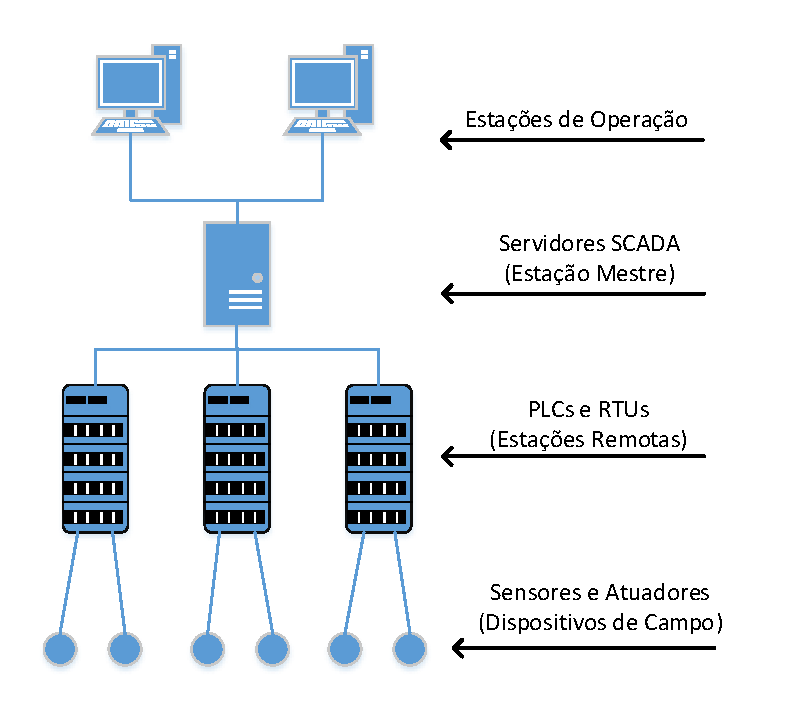
\includegraphics[scale=0.5]{pc_plc}  %pode alterar o tamanho
				\caption[Arquitetura do sistema instalado]{\label{fig:pc_plc}Arquitetura do sistema instalado. Adaptado de \textcite{pablo2011}}
			\end{center}		
		\end{figure}
	
		Dispositivos de campos podem ser entendidos pelos sensores e atuadores. Os sensores medem grandezas físicas do processo. enquanto os atuadores interferem no processo como por exemplo através  acionamento de bombas e válvulas. 
	
		As estações remotas são dispositivos programáveis que possuem a função de fazer a interface entre dispositivos de campo e estações mestre, além de serem dotados de capacidade de executar algoritmos de controle local. Nessa categoria enquadram-se os CLPs e RTUs. Os CLPs surgiram no contexto de chão de fábrica, ou seja, necessidade de programação e menor alcance de comunicação, devida a pequena distância entre os equipamentos. As RTUs surgiram da necessidade de enviar dados de sistemas localizados a grandes distâncias da estação mestre. Contudo, a evolução desses equipamentos tornou difícil a distinção entre eles \cite{bailey2003}.
		
		As estações mestres são o cérebro do sistema. Elas são responsáveis por solicitar dados das estações remotas, processá-los, armazená-los, bem como repassar comandos dos operadores para as estações remotas. As estações mestres são computadores, cuja capacidade depende do porte do projeto. Existem diferentes fabricantes de software que podem ser executados nesses servidores. Alguns fabricantes disponibilizam a opção de separar o processamento em diferentes estações mestres.
		
		As estações de operação executam um software que apresenta uma interface gráfica para o usuário, em que o operador consegue visualizar e interferir no processo através de controles (botões, sliders, etc) disponibilizados pela interface. Em pequenas aplicações, as estações de operação e as estações mestres se encontram nos mesmos computadores.
	
		A comunicação entre estação mestre e remota se dá pela utilização de protocolos industriais abertos como por exemplo Modbus\footnote{\url{http://www.modbus.org/}}, DNP3\footnote{\url{https://www.dnp.org/Default.aspx}}, OPC\footnote{\url{https://opcfoundation.org/about/what-is-opc/}}, entre outros; também há a comunicação através de protocolos proprietários. Este último caso ocorre em sua maioria quando a estação mestre e remota são fornecidos pelo mesmo fabricante.
	
	\subsection{Tecnologia Embarcada}
		Como mencionado no \autoref{cap:introducao}, os sistemas embarcados, estão cada vez mais presentes no setor industrial. \textcite{yu2011}, fazem uma pesquisa sobre os modelos de sistemas embarcados e em quais tipos de aplicações industriais estão sendo utilizados.
		
		Destacam-se a utilização de microcontroladores para executar algoritmos de controle e comunicação com outros sistemas. Um estudo de caso cita o túnel de vento instalado na Universidade de Bradley. A arquitetura do sistema implantado é mostrada na \autoref{fig:lab_view}. Comparando com a arquiteura SCADA descrita anteriormente, os elementos marcados com o número 1, seriam os dispositivos de campo, o microcontrolador (2), seria a estação remota, o PC executando o LabView (3) seria a estação master, e o outro computador seria a estação de visualização (IHM).
		
		\begin{figure}[!htb]	
			%\centering
			\captionsetup{justification=centering}
			\setlength{\belowcaptionskip}{-5pt}
			\begin{center}
				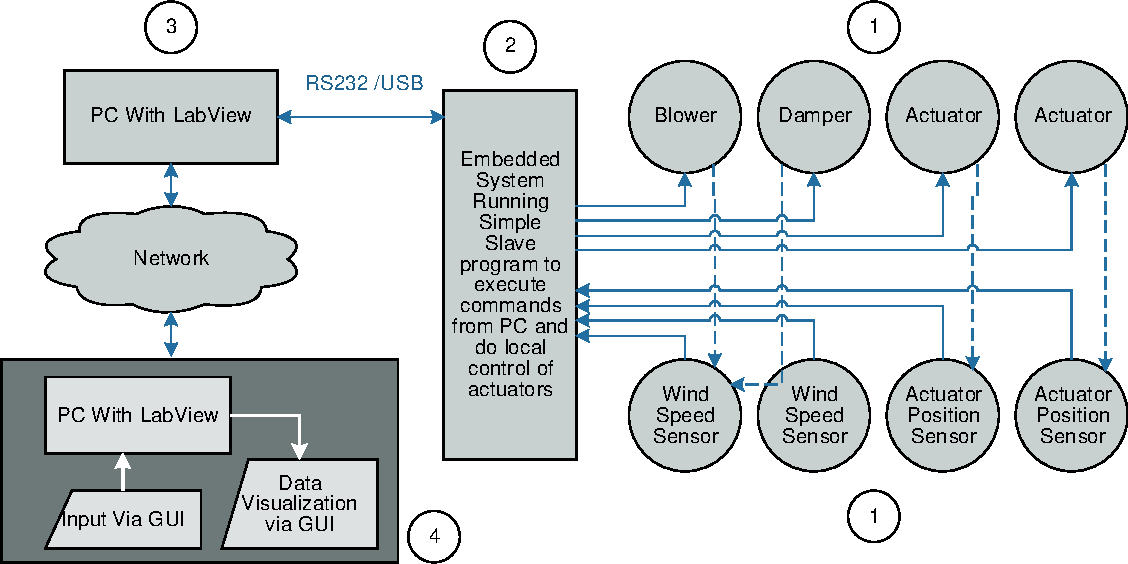
\includegraphics[width=15cm]{lab_view}  %pode alterar o tamanho
				\caption[Exemplo de Sistema com tecnologia embarcada]{\label{fig:lab_view}Exemplo de Sistema com tecnologia embarcada. Adaptado de \textcite{yu2011}}
			\end{center}		
		\end{figure}
	
		O estudo ainda menciona sobre crescimento da utilização de FPGAs\footnote{FPGAs e Microcontroladores: \url{https://www.7pcb.com/blog/fpgas-and-microcontrollers/}} em funções ocupadas pelos microcontroladores, devido a redução dos custos de aquisição dos mesmos, bem como pelas melhorias observadas em relação a capacidade de reconfiguração, o que facilita a sua utilização.
		
		É possível encontrar também diversos trabalhos na literatura que utilizam plataformas de prototipagem eletrônica para conceber projetos de automação para o setor residencial, para plantas de pequeno porte e para projetos na área educacional como plantas didáticas. A portabilidade é uma característica desejada para aplicações desses setores, que também são caracterizadas por possuírem restrições de custo, o que motiva a utilização de hardwares e softwares livres bem como ferramentas multiplataforma.
		
	\subsection{Plataformas de Prototipagem}
		O termo prototipagem rápida designa um conjunto de tecnologias utilizadas para fabricação de objetos físicos diretamente a partir de fontes de dados gerados por sistemas de projeto auxiliado por computador \cite{gorni2001}. A construção do objeto através da agregação de camadas permitem aos projetistas criar protótipos rapidamente.
		
		Este conceito pode ser extrapolado para o desenvolvimento dispositivos eletrônicos. Atualmente no mercado, encontram-se placas baseadas em microcontroladores e microprocessadores que podem se agregar a módulos, construindo assim, um novo produto. Essas placas são reprogramáveis, o que torna o processo de prototipagem rápido e flexível. A seguir serão apresentadas duas das principais placas de prototipagem do mercado.
		
	\subsubsection{Arduino}
		Arduino é uma plataforma eletrônica 	open-source baseado em hardware e sofware flexíveis e fáceis de usar \cite{arduino}. Basicamente a plataforma Arduino consiste em um conjunto de placas
		que possuem um microcontrolador, terminais de entradas e saídas analógicas, digitais e de dados, e uma porta para programação. Como se trata de um hardware livre, é possível que os usuários produzam as próprias placas.
		
		As placas se diferem pela arquitetura do microcontrolador, número de terminais, memória, entre outros. Uma placa pode ter as suas funcionalidades aumentadas através da inserção de Shields, que nada mais são que outras placas fabricadas com propósitos específicos. A placa Arduino UNO\footnote{\url{https://store.arduino.cc/usa/arduino-uno-rev3}} é uma das mais conhecidas, porém existem diversas placas mais poderosas, inclusive que suportam sistema operacional linux, como o Arduino Yun\footnote{\url{https://store.arduino.cc/usa/arduino-yun}}. Como mencionado anteriormente, foi utilizado o Arduino DUE no projeto, que está categorizada como uma das placas mais potentes e com maior número de terminais.
		
		Essa plataforma conta com inúmeras bibliotecas desenvolvidas pela comunidade usuária, que podem ser baixadas diretamente da página do Arduino, ou então disponibilizadas em páginas de compartilhamento de código open-source como o GitHub. A página do Arduino também disponibiliza uma IDE (Integrated Development Environment) para programação da placa. Se o usuário deseja programar em um nível mais baixo, como por exemplo acesso aos registradores internos do Arduino, é possível utilizar o Atmel Studio\footnote{\url{https://www.embarcados.com.br/atmel-studio/}}.
	
	\subsubsection{Raspberry PI}
		Um Raspberry PI é um computador de pequena dimensão (comparável com a dimensão de um cartão de crédito). O objetivo inicial da criação era criar um dispositivo de baixo custo para incentivar a prática de programação em níveis anteriores à graduação. Porém devido ao seu pequeno tamanho, baixo custo e razoável poder de processamento foi sendo adotado em muitos projetos eletrônicos. As placas Rasberry aceitam diversos sistemas operacionais, sendo que o sistema operacional oficial é o Raspian\footnote{\url{https://www.raspberrypi.org/downloads/raspbian}}, uma versão da distribuição Debian/Linux\footnote{\url{https://www.debian.org/}}. Ao longo dos anos, foram lançadas algumas versões das placas, que foram aumentando seu poder de processamento e inserindo mais funcionalidades. Um resumo das características das principais versões lançadas pode ser visto na \autoref{tbl:versoes_rpi}. Uma das grandes vantagens da versão 3, que foi a versão adquirida para o projeto é possuir os módulos Bluetooth e Wifi integrados à placa.
		
		\begin{table}[!htb]
			\centering
			\captionsetup{justification=centering}
			\caption[Comparação entre versões do Raspberry PI]{Comparação entre versões do Raspberry. \\Adaptado de \url{https://en.wikipedia.org/wiki/Raspberry_Pi}}
			\label{tbl:versoes_rpi}
			\def\arraystretch{1.3}
			\resizebox{\textwidth}{!}{
			\begin{tabularx}{\textwidth}{m{3.8 cm}| m{3cm} m{3cm} p{3cm}}
				& \multicolumn{1}{c}{\textbf{Raspberry 1}} & %\textbf{Raspberry 1+} & 
				\multicolumn{1}{c}{\textbf{Raspberry 2}} & \multicolumn{1}{c}{\textbf{Raspberry 3}} \\ \hline
				
				Lançamento & \multicolumn{1}{c}{02/2013} & %\multicolumn{1}{c}{07/2014} &
				\multicolumn{1}{c}{02/2015} & \multicolumn{1}{c}{02/2016} \\
				
				Preço & \multicolumn{1}{c}{\$25} & %\multicolumn{1}{c}{\$25} &
				\multicolumn{1}{c}{\$35} &
				\multicolumn{1}{c}{\$35} \\
				
				Arquitetura & \multicolumn{1}{c}{ARMv6Z} & %\multicolumn{1}{c}{ARMv6Z} &
				\multicolumn{1}{c}{ARMv7-A} &
				\multicolumn{1}{c}{ARMv8-A} \\
				
				CPU & \multicolumn{1}{c}{700Mhz one core} & %\multicolumn{1}{c}{700Mhz one core} &
				\multicolumn{1}{c}{900Mhz quad-core 64bit} &
				\multicolumn{1}{c}{1.2Ghz quad-core 64bit} \\
				
				Memória & \multicolumn{1}{c}{256MB} & 
				%\multicolumn{1}{c}{512MB} &
				\multicolumn{1}{c}{1GB} &
				\multicolumn{1}{c}{1GB} \\
				
				Nº de Portas USB & \multicolumn{1}{c}{1} &
				%\multicolumn{1}{c}{4} &
				\multicolumn{1}{c}{4} &
				\multicolumn{1}{c}{4} \\
				
				Corrente & \multicolumn{1}{c}{300mA} &
				%\multicolumn{1}{p{2cm}}{200mA - 350mA} &
				\multicolumn{1}{c}{220mA - 820mA} &
				\multicolumn{1}{c}{300mA - 1.34A} \\
				
				Wifi Integrado & \multicolumn{1}{c}{Não} & %\multicolumn{1}{c}{Não} &
				\multicolumn{1}{c}{Não} &
				\multicolumn{1}{c}{Sim. 802.11n} \\
				
				Bluetooth Integrado  & \multicolumn{1}{c}{Não} & %\multicolumn{1}{c}{Não} &
				\multicolumn{1}{c}{Não} &
				\multicolumn{1}{c}{Sim. v4.1} \\
				
				\hline
			\end{tabularx}}
		\end{table}
	
		O Raspberry possui um conjunto de pinos, que são úteis para realizar comunicação com outros dispositivos através de protocolos como UART, SPI e I2C, bem como enviar e receber informações digitais (nível lógico 0 ou 1) de dispositivos diversos. A \autoref{fig:gpio} mostra os componentes da placa Raspberry Pi 3, bem como uma breve explicação das funcionalidades dos 40 pinos. Observa-se que os pinos que são capazes de realizar comunicação são específicos. Outra informação importante é que os pinos lógicos suportam níveis de tensão até 3.3v, o que difere da tecnologia TTL tradicional, que suporta 5V. Ou seja, caso os pinos sejam submetidos a tensões de 5V, corre-se o risco de danificar a placa.
		
		\begin{figure}[!htb]	
			%\centering
			\captionsetup{justification=centering}
			\setlength{\belowcaptionskip}{-5pt}
			\begin{center}
				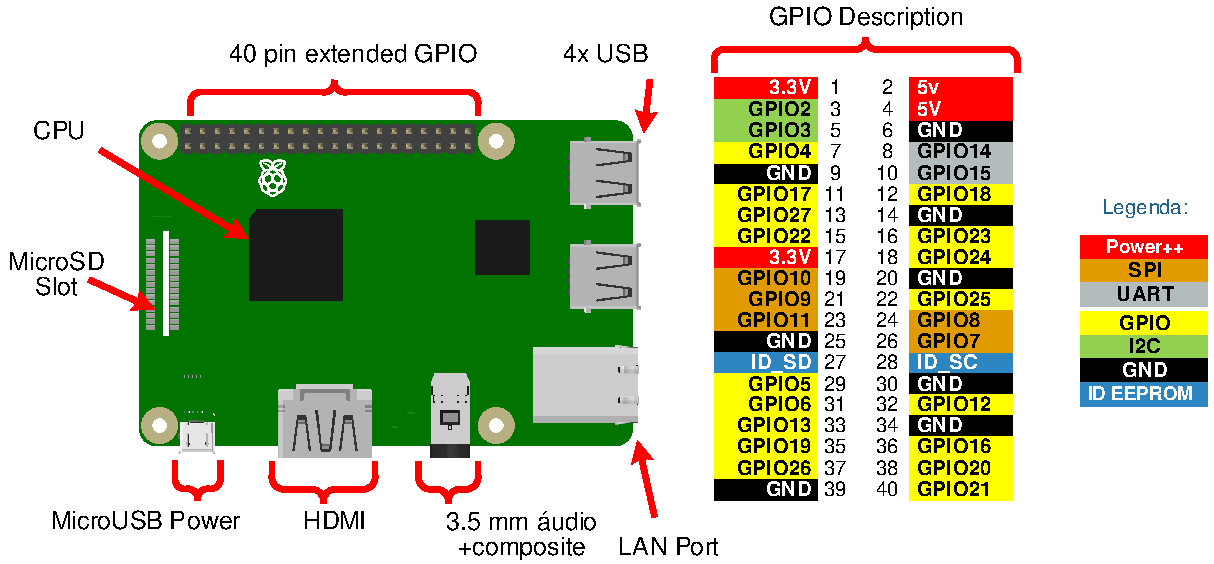
\includegraphics[width=15cm]{rpi_gpio}  %pode alterar o tamanho
				\caption[Composição de um Raspberry PI 3]{\label{fig:gpio}Composição de um Raspberry PI 3}
			\end{center}		
		\end{figure}
	
		\subsubsection{Protocolos de Comunicação}
			Um protocolo de comunicação consiste em um conjunto de regras e convenções criadas para possibilitar a comunicação entre dispositivos. Alguns exemplos de regras existentes em um protocolo: como um dispositivo identifica o outro, quando pode enviar e receber a informação, quanto tempo limite de espera por uma mensagem, entre outros \cite{lucas2016}.
			
			Existem alguns protocolos para estabelecer a comunicação entre Raspberry e Arduino. Basicamente, os protocolos são implementados por bibliotecas, que podem ser utilizadas por Raspberry e Arduino. Como é possível criar softwares em várias linguagens no Raspberry, as bibliotecas a serem utilizadas para esse dispositivo dependem da linguagem de programação utilizada.
			
			Como mostrado na \autoref{fig:gpio}, o Raspberry possui terminais para comunicação SPI, I2C, e UART. Estes protocolos também são suportados pelo Arduino. \textcite{robocore,kevin2015} apresentam um comparativo entre esses protocolos, cujas caracterísitcas estão descritas na \autoref{tbl:comparativo_protocolos}
			
		\begin{table}[!htb]
			\centering
			\captionsetup{justification=centering}
			\caption[Comparação entre SPI I2C e UART.]{Comparação entre SPI I2C e UART. Adaptado de \textcite{robocore}}
			\label{tbl:comparativo_protocolos}
			\def\arraystretch{1.5}
			\begin{tabular}{c c c c c c c}
				Protocolo & Taxa & Sentido & Método & Nº Fios & Tensão & Max \\ 
				& (bps)& Transmissão & & & & dispositivos \\ \hline
				UART & 1200 a 115200 & Full-Duplex & Assíncrono & 2 & 0 a 5V & 1 \\
				SPI & 0 a 10mb & Full-Duplex & Síncrono & 3+N & 0 a 5V & não há \\
				I2C & 100k ou 400k & Half-Duplex & Síncrono & 2 & 0 a 5V & 127 ou 1024 \\
				\hline
			\end{tabular}
		\end{table}
	
		O protocolo SPI possui  a vantagem de o mais rápido entre eles e também ser Full-Duplex. As desvantagens consistem em: aumento do número de fios à medida que o número de dispositivos na rede cresce; alguns dispositivos pode não suportar velocidades muito altas, o que pode causar incompatibilidade na comunicação; é mais suscetível a ruídos.
		
		O protocolo UART possui como vantagem a simplicidade das mensagens envolvidas na comunicação, bem como a sua disponibilidade em diversos dispositivos. Muitas vezes utilizam-se USB e RS-232 para trafegar dados em UART. Como desvantagem destaca-se: limitação em termos de velocidade; ser assíncrono, ou seja é necessário que a taxa de transmissão e recepção seja a mesma para ambos os dispositivos.
		
		O I2C se situa em uma região intermediária entre UART e SPI. É um protocolo síncrono, utiliza-se de apenas 2 fios, e possui uma taxa de transmissão um pouco maior que o UART. Como desvantagem, destaca-se a necessidade de interpretar os pacotes de dados via software, o que pode diminuir a performance de processamento.
		
		\subsubsection{Exemplos de Projetos que utilizaram Plataformas de Prototipagem}
			Encontra-se na literatura, projetos que utilizam placas de prototipagem mencionadas acima, para implementar um sistema de automação de pequenas instalações.
			
			\textcite{lucas2016} implementou a automação de uma planta experimental de um sistema de reaproveitamento de água. O modelo experimental foi construído, instalaram-se sensores e atuadores que se conectam a Arduino. O Arduino se comunica com um Raspberry PI, que possui um sofware SCADA instalado, o Mango automation. Ou seja, essa arquitetura é próxima a de um sistema SCADA tradicional, mostrada na \autoref{fig:pc_plc}. O Arduino faz o papel de uma estação remota, e o Raspberry, de uma estação mestre.
			
			Existe um projeto open-source de um sistema de controle de temperaturas para cervejarias chamado BrewPi \cite{brewpi}. O sistema consiste em um Raspberry PI que comunica com um Arduino, que é encapsulado a uma caixa que possui um display LCD para visualização de informações em modo local. O Arduino implementa algoritmos de controle em malha fechada, bem como possui funcionalidades para ler informações do processo, bem como acionar aquecedor e refrigerador. O Raspberry implementa um WebServer, que disponibiliza os dados do processo para os usuários. Para monitorar o processo, basta um dispositivo que possua um navegador Web. Fazendo um comparativo com a arquitetura SCADA tradicional, o WebServer seria o software SCADA que é executado nas estações mestres, e as estações de operação podem ser representadas por qualquer dispositivo com um navegador Web. Essa arquitetura concede portabilidade à operação, característica desejável a qualquer projeto. A arquitetura do sistema Brewpi é exibida na \autoref{fig:arq_brewpi}. Este projeto é um dos exemplos do crescimento da utilização de sistemas Web para monitoramento e controle de processos.
			
			\begin{figure}[!htb]	
				%\centering
				\captionsetup{justification=centering}
				\begin{center}
					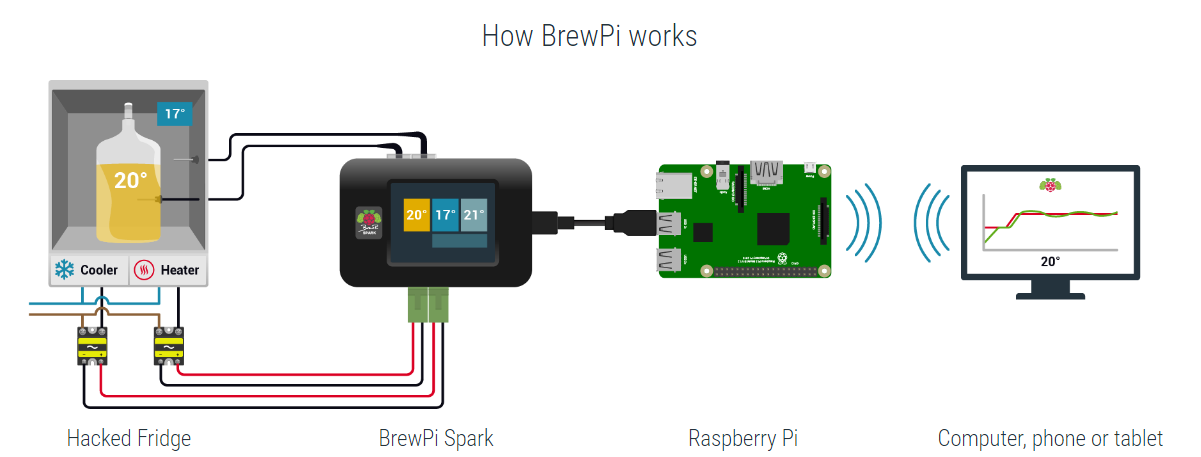
\includegraphics[width=14cm]{arq_brewpi}  %pode alterar o tamanho
					\caption[Arquitetura do sistema BrewPi]{\label{fig:arq_brewpi}Arquitetura do sistema BrewPi. Fonte: \url{https://www.brewpi.com/} }
				\end{center}		
			\end{figure}
		
	\section{Aplicações Web}
		A Web, abreviação do termo \textit{World Wide Web}, que significa em tradução livre ``rede de alcançe mundial'', também conhecida como www, é um sistema distribuído de hipermídia que revolucionou como pessoas organizações e sistemas geram, acessam e compartilham informações \cite{bernes2000}. Foi criada em 1989 por Tim Berners Lee resolver problemas em relação a transmissão e compartilhamento de informações do CERN (Organização Europeia para a pesquisa Nuclear).
		
		Porém o sucesso da Web fez com que a sua utilização não ficasse restrita ao meio acadêmico, sendo utilizada para fins pessoais e comerciais. O crescimento exponencial da Web causou um temor entre a comunidade e pesquisadores da internet, sobre a estabilidade da rede diante da crescente demanda. Diante disso, surgia a necessidade de melhorar a Web em termos de escalonabilidade performance e padronização em relação as aplicações. Em 1994 Berners-Lee fundou a W3C, órgão responsável pela padronização de tecnologias Web, instituição mais importante e reconhecida no mundo sobre o assunto \cite{felipe2008}.
		
		Ao longo dos anos, a Web sofreu transformações, em relação a aplicabilidade e a forma de transmitir informações. Inicialmente, as páginas Web publicavam apenas conteúdo estático, ou seja textos sem muita interatividade. O crescimento da Internet e o aumento da largura de banda fez com que fossem criados sites cada vez mais dinâmicos e interativos, incluindo a participação do internauta na geração de conteúdo, como por exemplo as redes sociais. Atualmente sistemas complexos que antes eram desenvolvidos apenas como aplicativos Desktop, podem ser criados utilizando somente tecnologias Web. A \autoref{fig:evolution_web} e a \autoref{fig:web_apps} exibem um resumo da evolução da web, suas tecnologias e aplicações.
		
		\begin{figure}[!htb]	
			%\centering
			\captionsetup{justification=centering}
			\begin{center}
				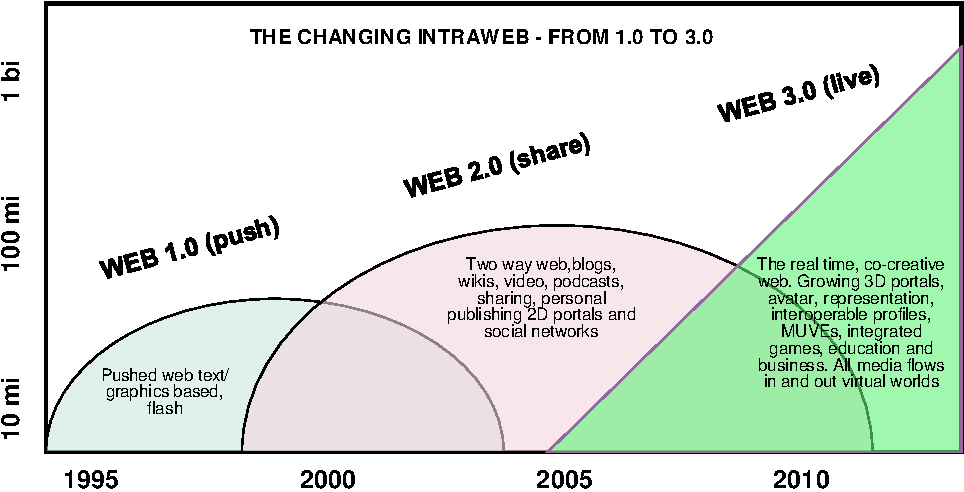
\includegraphics[scale=0.8]{evolution_web}  %pode alterar o tamanho
				\caption[Evolução da Web.]{\label{fig:evolution_web} Evolução da Web. Adaptado de \url{http://www.personalizemedia.com/virtual-worlds-web-30-and-portable-profiles/}}
			\end{center}		
		\end{figure}
	
		\begin{figure}[!htb]	
			%\centering
			\captionsetup{justification=centering}
			\begin{center}
				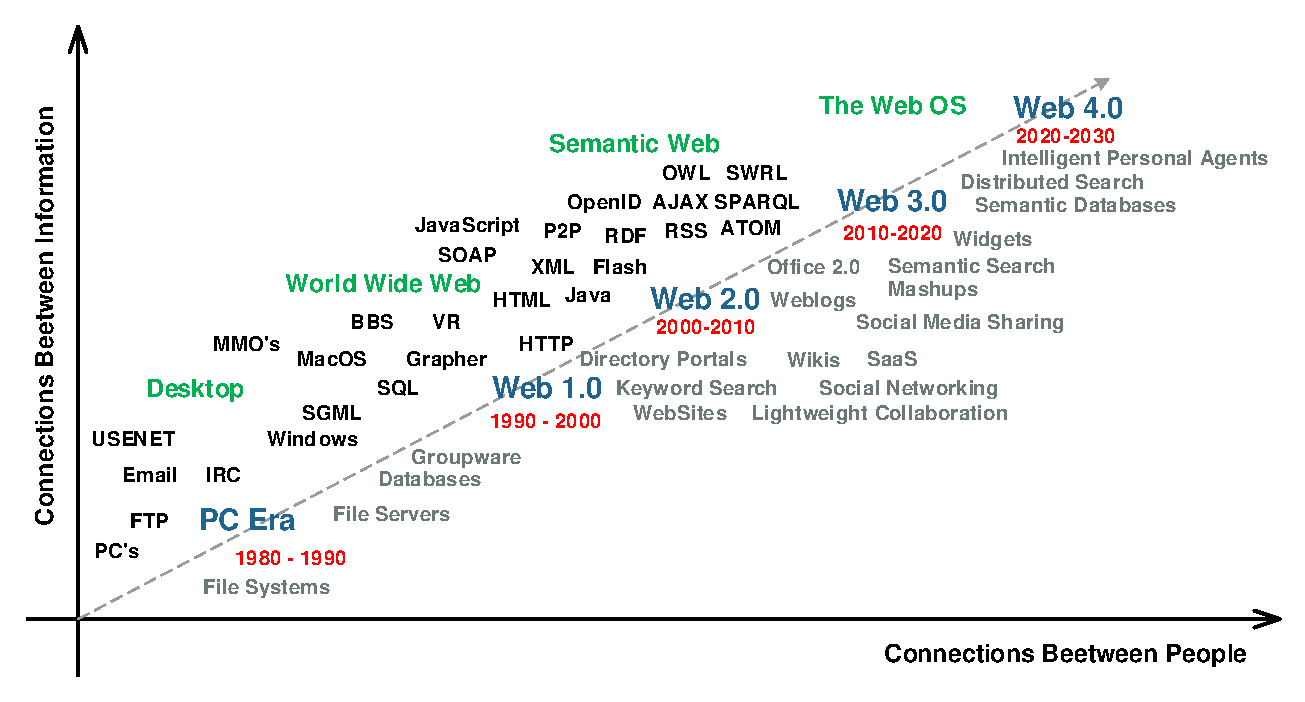
\includegraphics[width=16cm]{web_apps}  %pode alterar o tamanho
				\caption[Evolução da Web. Tecnologias e Aplicações]{\label{fig:web_apps} Evolução da Web. Tecnologias e Aplicações. Adaptado de \url{https://www.prokarma.com/blog/2014/10/16/what-exactly-web-30}}
			\end{center}		
		\end{figure}
		
		Uma aplicação Web tradicional é baseada em estilo cliente-servidor. Basicamente, um servidor oferece serviços e espera por requisições, enviadas por clientes interessados nesses serviços. Ao receberem as requisições, os servidores processam a requisição e enviam uma resposta ao cliente, que é representado por navegadores web. A \autoref{fig:request_response} mostra o fluxo de informações de uma requisição web e a resposta do servidor. As informações trafegam pelo protocolo HTTP\footnote{Especificação HTTP: \url{https://www.ietf.org/rfc/rfc2616.txt}}. Um frame HTTP de requisição possui a estrutura mostrada na \autoref{fig:http_frame}. O método GET é o mais utilizado. Ele possui a função de recuperar algum recurso, que é identificado por sua URL, do servidor Web. Existem outros métodos no protocolo HTTP, como POST, PUT, DELETE, etc \cite{diego2016}. O conteúdo a ser exibido nas páginas é produzido e armazenado em arquivos HTML, que basicamente é um arquivo de texto com marcações. Os navegadores interpretam os arquivos e exibem a página formatada para o usuário. Diante da característica dinâmica das páginas web atuais, outros arquivos se fazem necessários como arquivos JavaScript e arquivos CSS, que são arquivos processados nos navegadores.
		
		\begin{figure}[!htb]	
			%\centering
			\captionsetup{justification=centering}
			\begin{center}
				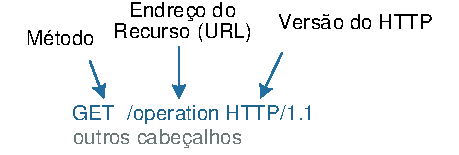
\includegraphics[scale=0.9]{http_frame}  %pode alterar o tamanho
				\caption[Frame de requisição HTTP]{\label{fig:http_frame} Frame de requisição HTTP}
			\end{center}		
		\end{figure}
	
		\begin{figure}[!htb]	
			%\centering
			\captionsetup{justification=centering}
			\begin{center}
				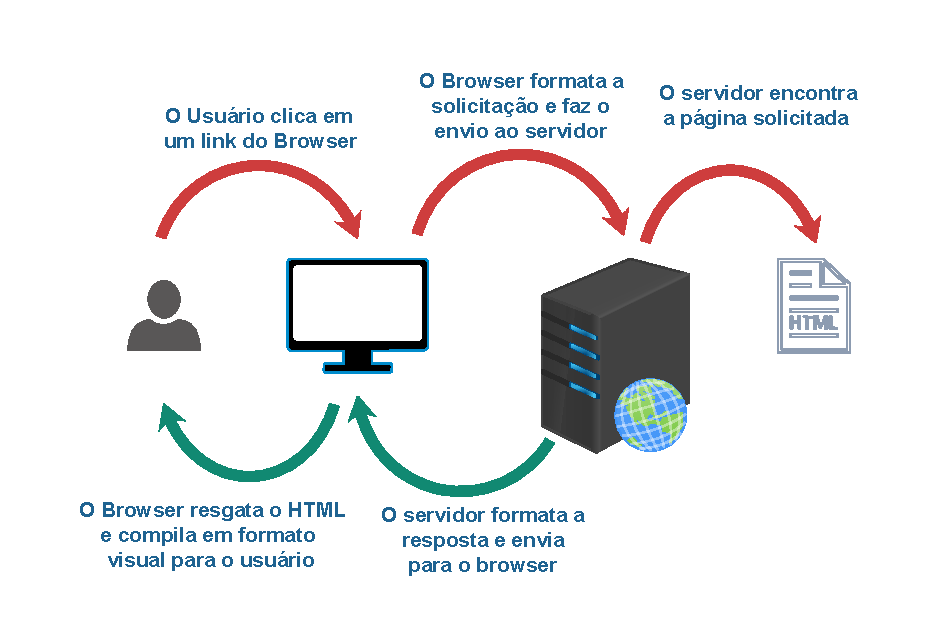
\includegraphics[scale=0.6]{request_response}  %pode alterar o tamanho
				\caption[Funcionamento do sistema requisição resposta.]{\label{fig:request_response} Funcionamento do sistema requisição resposta. Adaptado de \url{https://www.devmedia.com.br/como-funcionam-as-aplicacoes-web/25888}}
			\end{center}		
		\end{figure}
		
	\subsection{Frameworks Web}
		Um Framework Web é um framework\footnote{Definição de framework: \url{https://pt.wikipedia.org/wiki/Framework}} de software, designado para facilitar o desenvolvimento de aplicações web. Possui funções para automatizar tarefas comuns em aplicações web, como por exemplo acesso à banco de dados, gerenciamento de sessões de conexões, geração templates para geração de HTML, e mapeamento de rotas. Sendo assim, a utilização de um framework web torna o desenvolvimento de uma aplicação mais rápido e fácil. Existem frameworks Web para as mais diversas linguagens de programação, com características e funcionalidades distintas. A escolha do framework é subjetiva: depende do propósito da aplicação, conhecimento do desenvolvedor, entre outros fatores. A \autoref{fig:popular_frameworks} mostra um ranking dos Frameworks mais populares, baseado na avaliação do framework no Github, e no número de questões do mesmo presentes no StackOverflow.
		
		\begin{figure}[!htb]	
			%\centering
			\captionsetup{justification=centering}
			\begin{center}
				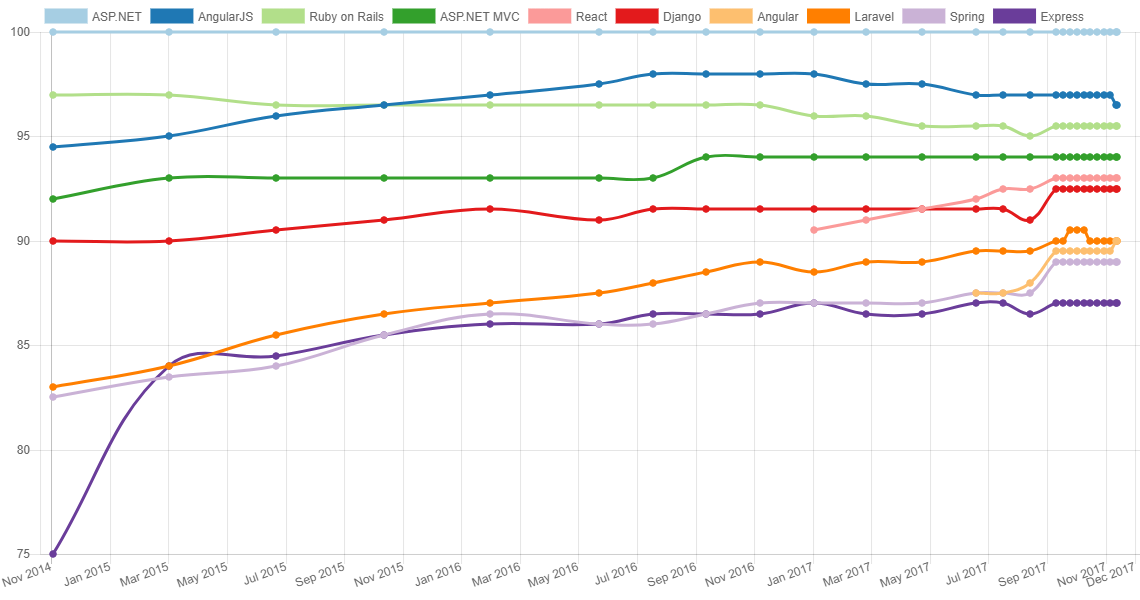
\includegraphics[width=14cm]{popular_frameworks}  %pode alterar o tamanho
				\caption[Frameworks Web mais populares]{\label{fig:popular_frameworks} Frameworks Web mais populares. Fonte: \url{https://hotframeworks.com/}}
			\end{center}		
		\end{figure}
	
	\subsubsection{Django}
		\label{sec:django}
		Django é um framework web desenvolvido na linguagem Python. É o framework mais utilizado escrito em Python, e um dos mais utilizados entre todas as linguagens (ver \autoref{fig:popular_frameworks}). Possui como características principais \cite{mozzila}: 
		\begin{enumerate}
			\item 
			Completude: O Django provê todas as funcionalidades básicas de uma aplicação web: compatibilidade com a maioria dos bancos de dados,
			recursos de proteção e segurança, controle de seções e cache,entre outros.
			\item 
			Versatilidade: O framework pode ser utilizado para desenvolver qualquer tipo de website. Consegue ser hospedado em vários servidores Web, bem como consegue trabalhar com qualquer framework para o lado cliente, como por exemplo o jquery\footnote{\url{https://jquery.com/}}.
			\item 
			Portabilidade: Como é escrito em Python, uma aplicação desenvolvida em Django pode ser hospedada nos principais sistemas operacionais (Linux, MacOS, Windows). 
			\item 
			Manutenibilidade: O framework foi concebido de acordo com princípios que incentivam a criação de códigos reutilizáveis e de fácil manutenção. Por exemplo, o django disponibiliza estruturas para implementar o DRY (Don't Repeat Yourself) filosofia que reduz a necessidade de replicação de código.
			\item 
			Escalabilidade: Um projeto desenvolvido em Django é composto de várias aplicações, que funcionam de forma independente entre si dentro do projeto. Essa separação entre partes do projeto permite além de flexibilidade (uma parte pode ser substituída ou modificada sem afetar o restante do código), crescimento escalável.
			\item
			Mapeamento Objeto-Relacional (ORM): É uma técnica que permite manipular dados de banco usando paradigma orientado a objetos. Basicamente, um modelo de dados é mapeado como uma tabela no banco de dados. Dessa forma elimina-se a necessidade de escrever códigos SQL para manipulação de bancos.
			\item 
			Popularidade: Possui uma extensa documentação e uma grande comunidade (em fóruns) disposta a ajudar.
		\end{enumerate}
	
		Como Django foi feito para possibilitar desenvolvimento rápido, muitas decisões de características do projeto fica a cargo do framework, o que é uma desvantagem. Outro ponto negativo é a geração de muitos arquivos mesmo para pequenos projetos.
		
		Um projeto em Django é criado sobre o padrão MVC\footnote{Padrão MVC: \url{https://developer.chrome.com/apps/app_frameworks}}, que em resumo é uma forma de programação que separa a representação da informação, do processamento dos dados em si. Dessa forma é possível possui por exemplo várias representações de uma mesma informação. A estrutura de uma aplicação em Django é exibida na \autoref{fig:django_project}.
			
		\begin{figure}[!htb]	
			%\centering
			\captionsetup{justification=centering}
			\begin{center}
				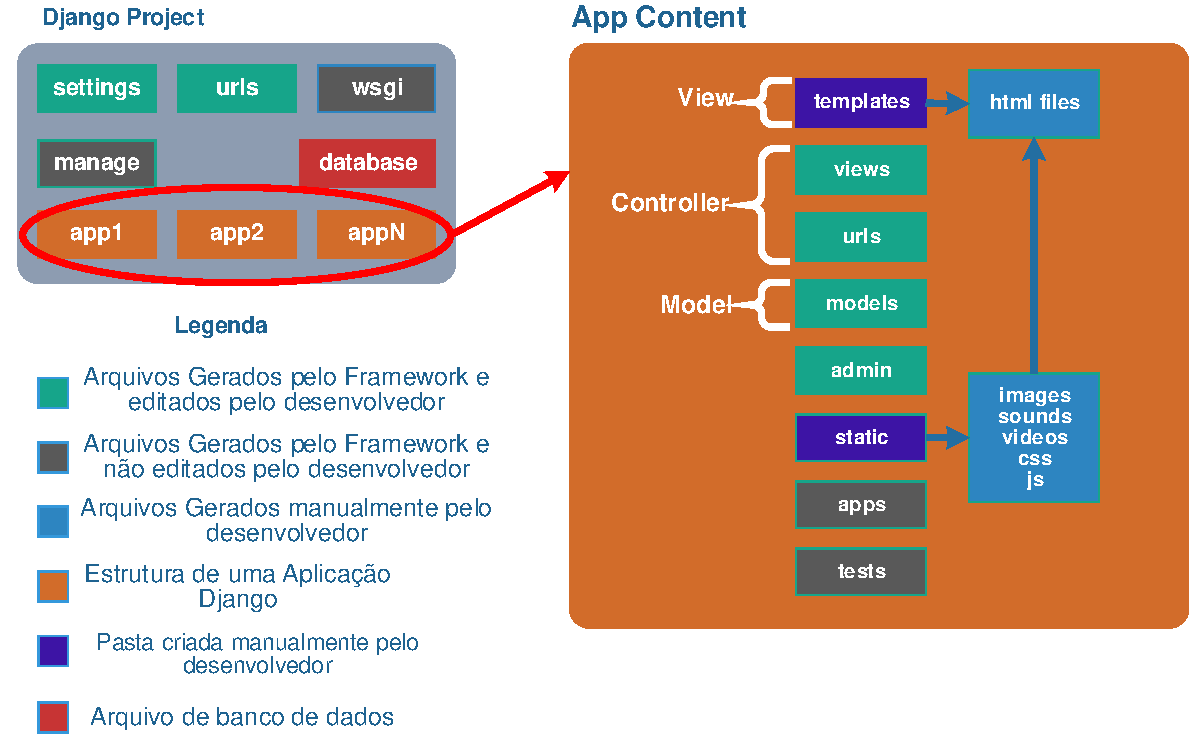
\includegraphics[width=14cm]{django_project}  %pode alterar o tamanho
				\caption[Estrutura de um projeto Django]{\label{fig:django_project} Estrutura de um projeto Django}
			\end{center}		
		\end{figure}
		
		
		

% ---
% Capitulo de Metodologia
% ---
\chapter{Metodologia}
	\chapterprecis{Este capítulo apresenta a arquitetura do sistema implementado. Primeiramente, são descritos os requisitos funcionais do sistema, que orientam a montagem da estrutura. São definidos os componentes do sistema e suas interconexões, sendo que esta definição é acompanhada de um breve descritivo do funcionamento.}
	
	\section{Estado Atual}
	
		A Arquitetura do sistema atual instalado na planta de trocador de calor está representada na \autoref{img3}. Pelo painel é possível efetuar a leitura das variáveis de processo, cuja leitura é feita pelo Arduino, bem como comandar a bomba e o aquecedor. É importante observar que o controle da potência do aquecedor não passa pelo Arduino, e que o sistema não recebe nenhum feedback sobre a velocidade da bomba, bem como sobre a potência do aquecedor. Apesar de estar previsto no projeto de \textcite{luiz2016}, nenhum controle em malha fechada está operacional.
		
		
	
		O intuito do projeto é implementar um sistema de monitoramento e controle remoto, sem que haja alteração infraestrutura já montada. Em resumo, o objetivo é implementar um sistema que necessite apenas se comunicar com o Arduino para executar as suas tarefas.
	
	
	\section{Requisitos Funcionais do Sistema}
		Para determinar a arquitetura do sistema a ser implementado, foram levantados os requisitos funcionais do sistema, ou seja, quais informações devem ser transmitidas ao operador, bem como quais as ações que este pode realizar no sistema. Os requisitos estão resumidos na \autoref{tbl1}.
		
		% Please add the following required packages to your document preamble:
		% \usepackage{booktabs}
		\begin{table}[!htb]
			\centering
			\caption{Requisitos Funcionais do Sistema}
			\label{tbl1}
			\def\arraystretch{1.3}
			\begin{tabular}{c p{11cm}}
				\hline
				\multicolumn{1}{c}{\textbf{Índice Requisito}} & \multicolumn{1}{c}{\textbf{Descrição Requisito}} \\ \hline 
				1 & Exibir a informação atual das variáveis de processo (vazões e temperaturas) \\ %\hline
				2 & Exibir o estado da bomba e do aquecedor (Ligado ou Desligado) \\ %\hline  
				3 & Exibir o valor da rotação atual da bomba \\ %\hline
				4 & Em modo remoto, deve permitir que o operador acione a bomba e o aquecedor \\ %\hline
				5 & Em modo remoto, deve permitir que o operador altere a velocidade da bomba \\ %\hline
				6 & Permitir a visualização dos dados analógicos em gráficos \\ %\hline
				7 & Impedir a atuação do operador quando o Arduino estiver em modo local ou de emergência \\ %\hline
				8 & Armazenar os dados do sistema em banco de dados \\ %\hline
				9 & Permitir que o usuário habilite ou desabilite o armazenamento de dados das variáveis \\ %\hline
				10 & Permitir que o usuário colete as informações contidas no banco em um arquivo no formato csv \\ %\hline
				11 & Permitir que o usuário apague as informações contidas no banco de dados \\ \hline
			\end{tabular}
		\end{table}
	
		Após levantamento dos requisitos, é possível concluir que as arquiteturas citadas na \autoref{sec:rev_monitor} podem ser utilizadas. É possível utilizar um PC que executa um software SCADA tradicional como utilizado por \textcite{alexandre2015}. Basicamente, o Arduino foi programado de forma que ele consiga utilizar um protocolo industrial comumente utilizado por ferramentas SCADA, no caso o protocolo Modbus\footnote{\url{http://www.ni.com/white-paper/52134/pt/}} foi utilizado. Também é possível utilizar uma arquitetura totalmente embarcada como utilizada no sistema \textit{BrewPi} \cite{brewpi}.
	
	\section{Critérios para Escolha do Sistema}
		Para possibilitar a comparação entre a arquitetura SCADA tradicional e embarcada e consequentemente ajudar na tomada de decisão, algumas características pontuais do sistema foram avaliadas. Existem características subjetivas e objetivas, sendo que as características subjetivas foram avaliadas de acordo com a experiência na utilização das ferramentas pelo desenvolvedor. Como existem diversos softwares SCADA no mercado, um software específico foi escolhido para comparação. O E3, que é fornecido pela Elipse Software\footnote{\url{https://www.elipse.com.br/produto/elipse-e3/}}, foi escolhido devido ao grau de conhecimento do desenvolvedor sobre a ferramenta. Os critérios e avaliações estão apresentados na \autoref{tbl2}.
		
		\begin{table}[!htb]
			\centering
			\caption{Comparação entre tecnologias}
			\label{tbl2}
			\def\arraystretch{1.5}
			\begin{tabularx}{\textwidth}{p{7cm} | c c}
				\hline
				\diagbox{\textbf{Critério}}{\textbf{Arquitetura}} & \multicolumn{1}{c}{\textbf{SCADA (E3)}} & \multicolumn{1}{p{5cm}}{\textbf{Tecnologia Embarcada}} \\ \hline
				
				\textcolor{blue}{Custo} & \multicolumn{1}{c}{Alto} & \multicolumn{1}{c}{Baixo} \\
				
				\textcolor{blue}{Complexidade do desenvolvimento das interfaces gráficas} & \multicolumn{1}{c}{Baixa} & \multicolumn{1}{c}{Alta} \\
				
				\textcolor{blue}{Complexidade da implementação da comunicação com Arduino} & \multicolumn{1}{c}{Baixa} & \multicolumn{1}{c}{Média} \\
				
				\textcolor{blue}{Facilidade para interoperar com outros sistemas} & \multicolumn{1}{c}{Média} & \multicolumn{1}{c}{Alta} \\ 
				
				\textcolor{blue}{Multiplataforma} & \multicolumn{1}{c}{Não} & \multicolumn{1}{c}{Sim} \\
				
				\textcolor{blue}{Interface se adapta à resolução do dispositivo} & \multicolumn{1}{c}{Não} & \multicolumn{1}{c}{Sim} \\
				
				\textcolor{blue}{Suporte a vários clientes conectados simultaneamente} & \multicolumn{1}{c}{Sim} & \multicolumn{1}{c}{Sim} \\
				
				\textcolor{blue}{Consumo de energia} & \multicolumn{1}{c}{Médio} & \multicolumn{1}{c}{Baixo} \\
						
				\hline
			\end{tabularx}
		\end{table}
	
		A grande disparidade entre esses sistemas basicamente é o custo em a relação a demanda de mão-de-obra especializada para desenvolvimento de sistemas embarcados. Conhecimentos de ferramentas SCADAs já estão difundidos, facilitando o desenvolvimento de aplicações utilizando essas ferramentas. Contudo, esses softwares são caros, com exceção de algumas ferramentas \textit{opensource} como por exemplo o SCADABR\footnote{\url{http://www.scadabr.com.br/}}.
		
		Desde o início da modernização do laboratório, o custo era uma das restrições mais fortes, o que favoreceu a opção pela tecnologia embarcada. Além disso, a oportunidade de utilizar tecnologias emergentes no monitoramento de processos contribuiu ainda mais para a utilização de sistemas embarcados.
		
	\section{Arquitetura do Sistema}
		A arquitetura pensada para o sistema foi inspirada no projeto BrewPi. Esse sistema foi concebido para controlar a temperatura de um recipiente com líquido, bem como para permitir o monitoramento via qualquer dispositivo que possua um navegador Web. A Arquitetura deste sistema é mostrada na \autoref{fig:arq_brewpi}. Basicamente, o Arduino, é encarregado de executar a malha de controle e enviar as informações para um RaspberryPi, que implementa um WebServer. Os usuários que desejam visualizar e/ou modificar as informações, devem abrir um navegador e se conectar ao WebServer para obter os dados.
		
		\begin{figure}[!htb]	
			%\centering
			\captionsetup{justification=centering}
			\begin{center}
				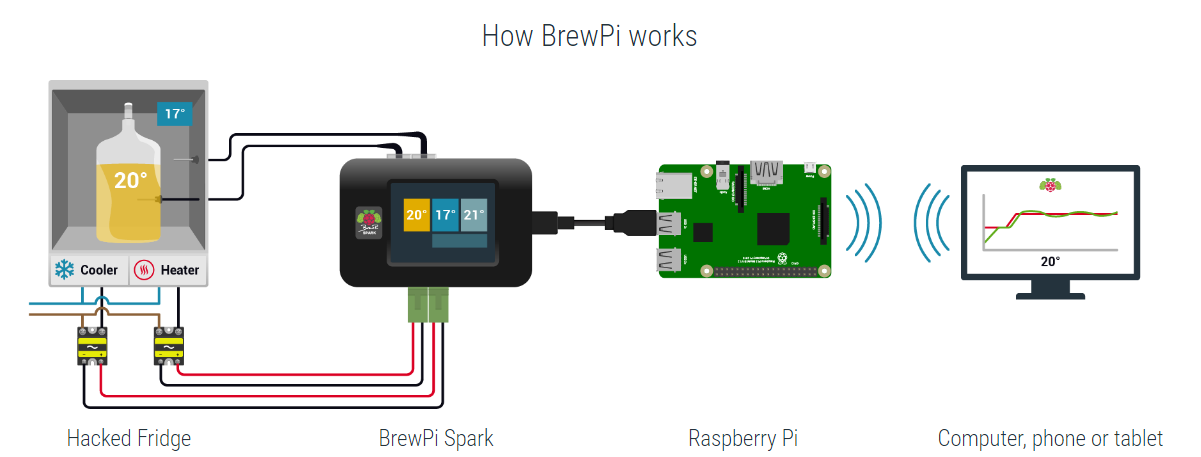
\includegraphics[width=14cm]{arq_brewpi}  %pode alterar o tamanho
				\caption[Arquitetura do sistema BrewPi]{\label{fig:arq_brewpi}Arquitetura do sistema BrewPi. Fonte: \url{https://www.brewpi.com/} }
			\end{center}		
		\end{figure}
	
		Para o trocador de calor, a proposta é semelhante. A adição de um RaspberryPi no sistema atual é simples de ser realizada e está em conformidade com a condição de não modificar as instalações atuais. Dessa forma, a arquitetura proposta simplificada para o sistema com o Raspberry é exibida na \autoref{fig:arq_proposta}. A Arquitetura detalhada do sistema, como por exemplo, os softwares a serem desenvolvidos em cada dispositivo, bem como a forma de interação entre eles serão tópicos abordados posteriormente.
		
		\begin{figure}[!htb]	
			%\centering
			\captionsetup{justification=centering}
			\begin{center}
				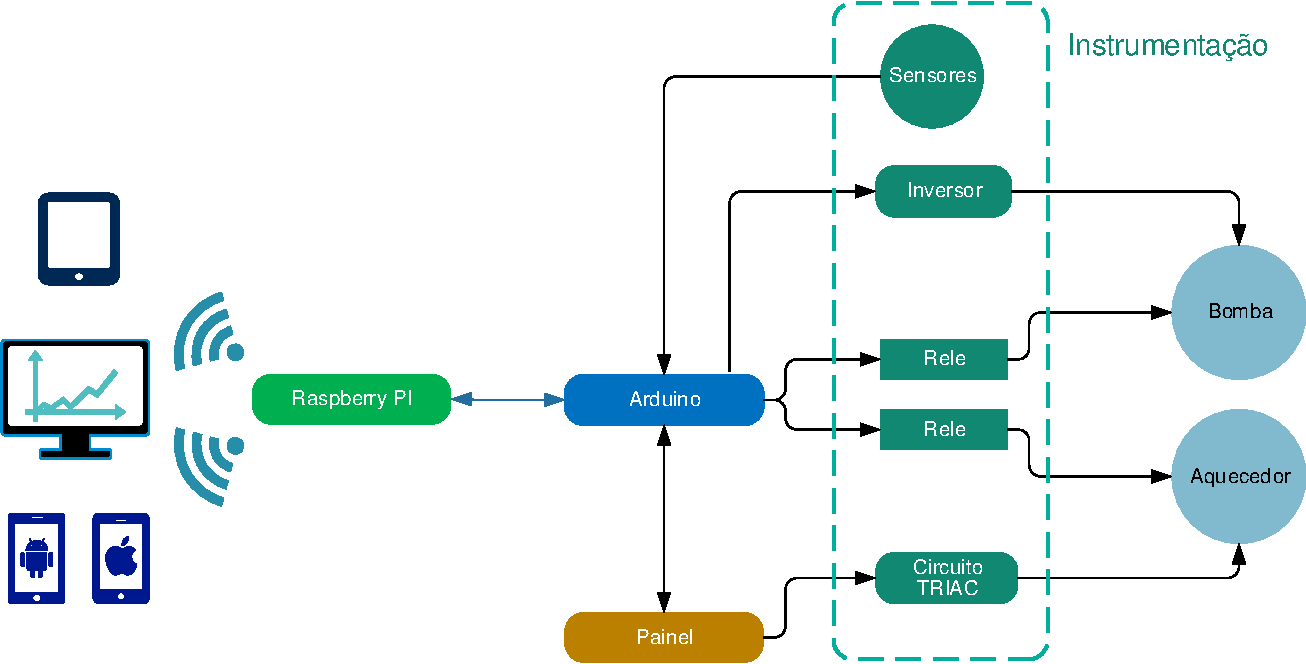
\includegraphics[width=14cm]{arq_proposta}  %pode alterar o tamanho
				\caption[Nova Arquitetura Proposta para o Sistema]{\label{fig:arq_proposta} Nova Arquitetura Proposta para o Sistema }
			\end{center}		
		\end{figure}
		
		É importante salientar que existem outros dispositivos simulares ao Raspberry PI como o BeagleBone Black\footnote{\url{https://beagleboard.org/black}} e a recente e também poderosa placa DragonBoard 410c\footnote{\url{https://developer.qualcomm.com/hardware/dragonboard-410c}}. Qualquer uma das placas poderia ser utilizada no projeto. A escolha do Raspberry PI foi influenciada pela extensa base de conhecimento e documentação já produzida pelos usuários, aliado ao menor custo da placa.  As demais placas por serem mais novas, não dispõem de muitos documentos e exemplos, o que aumenta o tempo de desenvolvimento de um novo projeto.
		
		Ainda em relação as placas utilizadas, verifica-se que existem vários modelos distintos de Raspberry PI. Portanto é necessário definir qual a versão é a mais adequada ao projeto.
		
		\subsection{Escolha da Versão do Raspberry PI}
			O Raspberry PI possui algumas versões, que se diferem em tamanho, capacidade de memória, processamento e componentes. Um resumo das características das principais versões do Raspberry é exibido na \autoref{tbl3}
			
			\begin{table}[!htb]
				\centering
				\captionsetup{justification=centering}
				\caption[Comparação entre versões do Raspberry PI]{Comparação entre versões do Raspberry. \\Adaptado de \url{https://en.wikipedia.org/wiki/Raspberry_Pi}}
				\label{tbl3}
				\def\arraystretch{1.5}
				\begin{tabularx}{\textwidth}{m{2.5 cm}| m{3cm} m{3cm} p{3cm}}
					  & \multicolumn{1}{c}{\textbf{Raspberry 1}} & %\textbf{Raspberry 1+} & 
					 \multicolumn{1}{c}{\textbf{Raspberry 2}} & \multicolumn{1}{c}{\textbf{Raspberry 3}} \\ \hline
					 
					 Lançamento & \multicolumn{1}{c}{02/2013} & %\multicolumn{1}{c}{07/2014} &
					 \multicolumn{1}{c}{02/2015} & \multicolumn{1}{c}{02/2016} \\
					 
					 Preço & \multicolumn{1}{c}{\$25} & %\multicolumn{1}{c}{\$25} &
					 \multicolumn{1}{c}{\$35} &
					 \multicolumn{1}{c}{\$35} \\
					 
					 Arquitetura & \multicolumn{1}{c}{ARMv6Z} & %\multicolumn{1}{c}{ARMv6Z} &
					 \multicolumn{1}{c}{ARMv7-A} &
					 \multicolumn{1}{c}{ARMv8-A} \\
					 
					 CPU & \multicolumn{1}{c}{700Mhz one core} & %\multicolumn{1}{c}{700Mhz one core} &
					 \multicolumn{1}{c}{900Mhz quad-core 64bit} &
					 \multicolumn{1}{c}{1.2Ghz quad-core 64bit} \\
					 
					 Memória & \multicolumn{1}{c}{256MB} & 
					 %\multicolumn{1}{c}{512MB} &
					 \multicolumn{1}{c}{1GB} &
					 \multicolumn{1}{c}{1GB} \\
					 
					 Nº de Portas USB & \multicolumn{1}{c}{1} &
					 %\multicolumn{1}{c}{4} &
					 \multicolumn{1}{c}{4} &
					 \multicolumn{1}{c}{4} \\
					 
					 Corrente & \multicolumn{1}{c}{300mA} &
					 %\multicolumn{1}{p{2cm}}{200mA - 350mA} &
					 \multicolumn{1}{c}{220mA - 820mA} &
					 \multicolumn{1}{c}{300mA - 1.34A} \\
					 
					 Wifi Integrado & \multicolumn{1}{c}{Não} & %\multicolumn{1}{c}{Não} &
					 \multicolumn{1}{c}{Não} &
					 \multicolumn{1}{c}{Sim. 802.11n} \\
					 
					 Bluetooth Integrado  & \multicolumn{1}{c}{Não} & %\multicolumn{1}{c}{Não} &
					 \multicolumn{1}{c}{Não} &
					 \multicolumn{1}{c}{Sim. v4.1} \\
					 
					\hline
				\end{tabularx}
			\end{table}
		
			A última versão do Raspberry apresenta uma grande vantagem por possuir Wifi nativamente. Isso evita a utilização de adaptadores para utilizar a comunicação Wireless no dispositivo. Além disso, possui maior poder de processamento, conta com um chip mais moderno, e suporta uma capacidade maior de corrente em estado de sobrecarga. Portanto, o Raspberry 3 foi escolhido. Na próxima seção detalhados os sistemas a serem executados dentro do Raspberry e como estes se relacionam entre si e com o Arduino.
			
		\subsection{Arquitetura Detalhada do Sistema}
			A \autoref{img3} exibe a visão geral do sistema, ou seja, não exibe como é a comunicação entre os componentes. Como dito anteriormente, não faz parte do escopo do projeto promover alterações nas instalações atuais, portanto, é necessário focar apenas em como o Raspberry será programado e como será realizada a sua comunicação com o Arduino.
			
			Os componentes foram projetados de forma que cada um funcione da forma mais independente possível. Dessa forma, o impacto no sistema caso haja alguma alteração de componente, em termos de esforço de desenvolvimento, é minimizado.
			
			A arquitetura detalhada do sistema é exibida na \autoref{fig:arq_componentes}. Foram definidos 3 componentes: o programa que é executado no Arduino; o Gateway e o WebServer, \textcolor{red}{que são} programas que são executados no Raspberry. O termo componente deve ser entendido nesse contexto como um programa, por isso o banco de dados não deve ser interpretado como um componente. Optou-se por criar dois programas no Raspberry PI, de forma que as funcionalidades do sistema fossem corretamente agrupadas. As atribuições de cada programa estão resumidas na \autoref{tbl4}
			
			\begin{table}[!htb]
				\centering
				\captionsetup{justification=centering}
				\caption[Atribuições de cada Componente]{Atribuições de cada Componente}
				\label{tbl4}
				\def\arraystretch{1.5}
				\begin{tabular}{m{2cm}| p{12cm}}
					& \multicolumn{1}{c}{\textbf{Atribuições}} \\ \hline
					
					\multirow{4}{*}{Arduino} 
					& 1 - Interface com sensores e Atudadores \\
					& 2 - Interface com Painel \\
					& 3 - Enviar estado do sistema quando solicitado pelo Gateway\\
					& 4 - Interpretar comandos enviados pelo Gateway \\ \hline
					
					\multirow{3}{*}{Gateway} & 5 - Solicitar de forma cíclica o estado das variáveis \\
					& 6 - Armazenar os dados recebidos em um banco de dados \\
					& 7 - Receber comandos vêm do WebServer (comandos dos usuários) e repassar ao Arduino \\ \hline
					
					\multirow{2}{*}{WebServer} & 8 - Ler dados do banco e apresentar ao usuário \\
					& 9 - Receber comandos do usuário e repassar ao Gateway \\
						
					\hline
				\end{tabular}
			\end{table}
			
			\begin{figure}[!htb]	
				%\centering
				\captionsetup{justification=centering}
				\begin{center}
					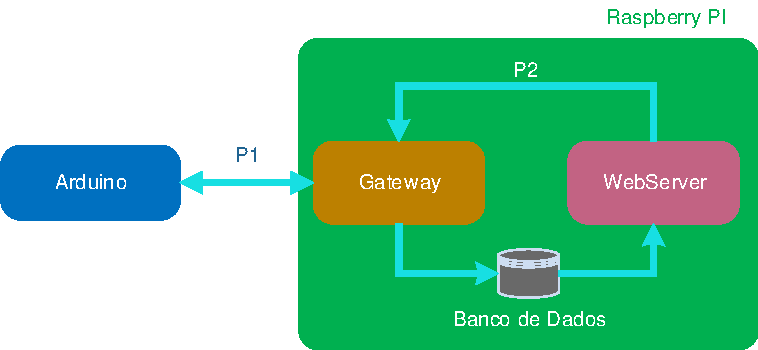
\includegraphics[width=12cm]{arq_componentes}  %pode alterar o tamanho
					\caption[Arquitetura Detalhada]{\label{fig:arq_componentes} Arquitetura Detalhada }
				\end{center}		
			\end{figure}
		
			É importante observar que as atribuições 4 e 5 envolvem uma comunicação entre Arduino e Gateway, e as atribuições 7 e 9 envolvem uma comunicação entre o WebServer e Gateway. Portanto, é necessário definir protocolos de comunicação para ambos os casos. Já foi dito que os componentes foram projetados de forma a possibilitar a substituição de um componente sem alterar os demais. Porém, alterações no protocolo de comunicação necessariamente levam a modificações nos componentes envolvidos. Em resumo, os protocolos de comunicação devem ser mantidos.
			
			
			\subsubsection{Funcionamento do Arduino}
				\label{sec:met_arduino}
				Foi feita uma análise do programa atual que o Arduino executa. O programa é extenso (contém 1482 linhas), sendo que cerca de 90\% do código é dedicado a cuidar do sistema de navegação do display LCD através dos botões existentes no painel.  A implementação de um sistema de monitoramento elimina a necessidade dessa estrutura de navegação, de modo que o painel passe a ter apenas funcionalidades diretas de acionamento, e o display exiba apenas informações básicas. Portanto, a melhor opção foi reformular o código do Arduino e aproveitar apenas as funções que fazem a leitura dos sensores e convertem os valores para unidade de engenharia.
				
				A estrutura do código, que está exibida na \autoref{fig:fluxo_arduino}, foi montada de forma a permitir rápida adaptação do mesmo para diferentes protocolos de comunicação, e está de acordo com as atribuições mencionadas na \autoref{tbl4}. As trocas de mensagens com o Gateway são feitas por interrupção, ou seja, estão fora da função \textit{loop} do Arduino. 
				
				O programa criado seguiu o paradigma de programação procedural, ou seja, o programa foi bastante modularizado. Esse tipo de prática acelera a identificação de uma funcionalidade (atribuição) no código fonte, o que facilita a manutenção deste. Outro benefício é a possibilidade de expansão de funcionalidades, como por exemplo a implementação de malhas de controle no código. \textcolor{red}{ Para isso, um Estado Automático cujas atribuições fossem executar as malhas de controle poderia ser adicionado ao sistema. Para que este estado entre em funcionamento, bastaria adicionar mais uma condição de teste no código, ou seja, uma alteração bastante simples.}
				
				No diagrama é utilizado o termo ``estado do sistema'', que deve ser interpretado como o conjunto de variáveis necessários para descrever o sistema. Essas variáveis são: as 4 temperaturas; 2 vazões; estado de acionamento de bomba e aquecedor (Ligado ou Desligado); velocidade da bomba; modo de operação (Local ou Remoto) e se o botão de emergência está acionado ou não.
			
				\begin{figure}[!htb]	
					%\centering
					\captionsetup{justification=centering}
					\begin{center}
						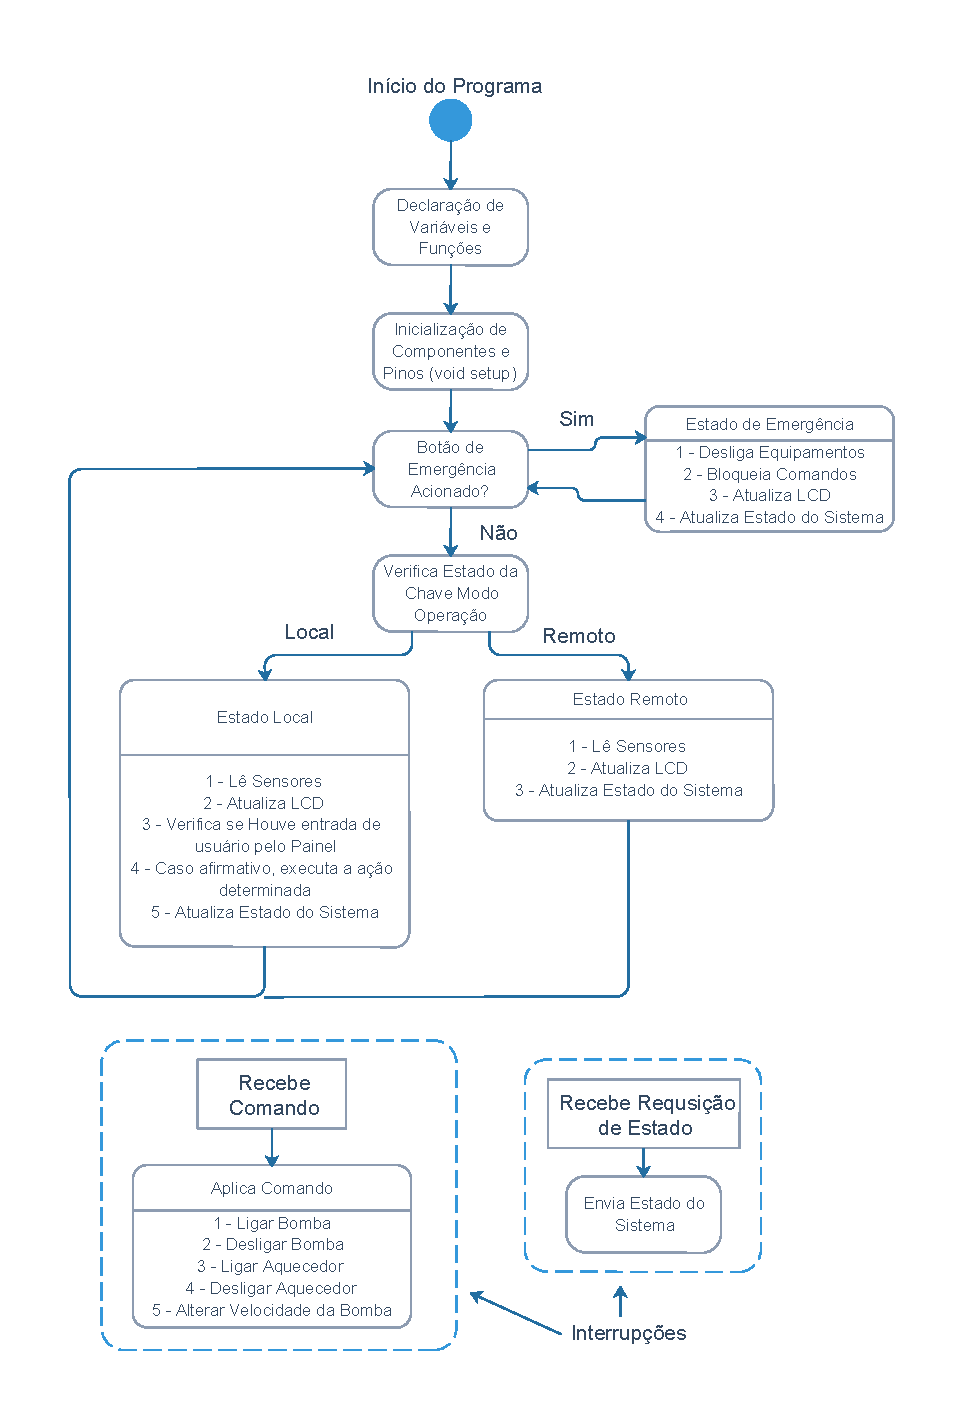
\includegraphics[width=12cm]{fluxo_arduino}  %pode alterar o tamanho
						\caption[Estrutura do Código do Arduino]{\label{fig:fluxo_arduino} Estrutura do Código do Arduino }
					\end{center}		
				\end{figure}
			
			\subsubsection{Comunicação Entre Arduino e Gateway}
				Ao observar as atribuições 3 e 4 da \autoref{tbl4}, verifica-se que a comunicação entre Arduino e Gateway é do tipo mestre-escravo, ou seja, o dispositivo mestre (Gateway) sempre inicia a comunicação, e o escravo (Arduino) responde quando solicitado. Existem diversos protocolos que implementam esse tipo de comunicação.
				
				É necessário escolher um protocolo que funcione em meio físico serial, uma vez que nenhum \textit{Shield} Ethernet será utilizado. É possível portanto utilizar algum protocolo industrial, disponibilizado na forma de bibliotecas, ou então algum dos protocolos seriais descritos na seção \textcolor{red}{colocar aqui a seção da rev sobre protocolos}, ou seja: UART, SPI, I2C.
				
				O protocolo industrial aberto encontrado com maior frequência em outras referências e implementações é o Modbus. É possível baixar pelo menos 5 bibliotecas que implementam o protocolo. A utilização de Modbus apresenta a vantagem de facilitar a integração com diferentes sistemas, uma vez que é um protocolo amplamente difundido e utilizado. Contudo, ao adicionar a biblioteca Modbus no Arduino, o código aumenta consideravelmente o tamanho, pois as bibliotecas implementam praticamente todo o protocolo, o que é desnecessário para o projeto atual, uma vez que a quantidade de informações trafegadas entre os componentes é pequena.
				
				O protocolo SPI possui uma taxa de transferência máxima maior que I2C e UART, porém a implementação da troca das mensagens entre os dispositivos é a mais complexa. O protocolo SPI exige o recebimento de informação enquanto está enviando, o que é ruim em para o propósito desse sistema, pois torna-se necessário o tratamento de informações indesejadas. A comunicação UART permite a implementação mais simples de troca de mensagens. Porém, é a mais lenta das 3, além de ser assíncrona. Além disso, a troca de mensagens é através de strings, portanto, o tamanho dos frames envolvidos na troca de mensagens é maior. 
				
				O protocolo I2C se apresenta como um meio termo entre SPI e UART, em termos de complexidade das trocas de mensagens e velocidade de comunicação. Além disso, é um protocolo síncrono, e a velocidade típica de utilização, que é 100kbps, atende plenamente ao projeto.
				Portanto, o I2C será utilizado no projeto. Existe uma biblioteca nativa que implementa o I2C para o Arduino, bem como existem bibliotecas I2C para diversas linguagens de programação (necessário para o Gateway). Os detalhes dos frames de comunicação serão explorados no capitulo de \textcolor{red}{implementação}.
			
			\subsubsection{Funcionamento do Gateway}
				\label{sec:met_gateway}
				O programa do Gateway foi desenvolvido em Python, embora possa ser escrito também em Java e C/C++, que são linguagens também suportadas pelo Raspberry. O Python foi escolhido por ser uma linguagem de programação de alto nível, ou seja, uma linguagem que está próxima da linguística humana. Essa característica facilita o entendimento de programas, e acelera o processo de aprendizado da mesma.
				
				O processo do Gateway foi dividido em duas Threads. Uma thread é responsável por solicitar os dados do arduino e enviar ao banco de dados, e a outra responsável por aguardar comandos vindos do WebServer, e repassar ao Arduino. A divisão se mostra uma decisão acertada. Enquanto a tarefa de leitura dos dados e envio ao banco é executada em um intervalo fixo, o recebimento dos dados do WebServer é essencialmente assíncrono, pois os usuários podem enviar comandos em qualquer momento. Portanto, implementar ambas as funcionalidades em uma única Thread seria inviável. Além disso, essa implementação permite o repasse do comando enviado pelo WebServer para o Arduino tão logo a mensagem seja recebida. As Threads compartilham apenas um recurso, que é o canal I2C, para escrita e leitura dos dados para o Arduino.
				
				\textcolor{red}{Vale a pena colocar uma imagem para ilustrar o que foi dito no texto?}
			
			\subsubsection{Comunicação entre WebServer e Gateway}
				A comunicação entre WebServer e Gateway é feita via TCP/IP. Uma das threads do Gateway implementa um servidor TCP assíncrono que fica ``escutando'' em uma determinada porta. A cada comando de usuário, o WebServer abre um cliente, se conecta ao servidor TCP, envia a informação necessária e posteriormente fecha a conexão. Dessa forma, evita-se manter conexões estabelecidas de forma desnecessária. A linguagem Python possui pacotes que implementam servidores e clientes TCP, ou seja, o desenvolvedor não necessita se preocupar com detalhes de implementação do protocolo. Sendo assim, o foco está apenas no conteúdo das mensagens envolvidas.
				
				As mensagens trafegadas consistem em um conjunto strings. Para simplificar o processo de decodificação da mensagem, bem como facilitar a captura de erros no transporte, decidiu-se transmitir as informações em pacotes JSON. Como dito na seção \textcolor{red}{colocar aqui a seção que fala sobre json}, uma das vantagens de se utilizar JSON é a fácil interpretação das mensagens, tanto pelos humanos, quanto pelos softwares.
				
			\subsubsection{WebServer}
				Conforme foi abordado na seção \textcolor{red}{colocar a seção sobre frameworks web}, existem frameworks web para diversas linguagens de programação, inclusive existem muitos frameworks para uma mesma linguagem de programação. A linguagem Python foi mantida para o desenvolvimento do WebServer, pelos mesmos motivos mencionados na seção anterior.
				
				\textcite{bogdan2017} e \textcite{ryan2015} abordam sobre as diferenças entre os diversos frameworks web existentes para a linguagem Python. O framework escolhido foi o Django devido a 4 motivos: 
				
				\begin{enumerate}
					\item 
					É um dos frameworks mais utilizados. Portanto, conta com uma vasta e completa documentação. 
					\item 
					A complexidade de uma aplicação escrita em Django é praticamente uniforme. Ou seja, uma aplicação de pequeno porte ou grande porte, resultam em um código de complexidade próxima.
					\item 
					O framework Django é adequado para usuários	que querem desenvolver aplicações web rapidamente, sem fazer muitas decisões sobre a infraestrutura da aplicação. Ou seja, o Django já fornece uma infraestrutura básica para possibilitar desenvolvimento imediato
					\item 
					Consultas a banco de dados não precisam ser feitas utilizando código SQL. O Django provê uma estrutura de forma que é possível manipular dados do banco através de códigos Python. Isso facilita, por exemplo, algumas funcionalidades do Gateway.
				\end{enumerate}
			
				Para apresentação da interface para o cliente são utilizadas as linguagens HTML e CSS. A parte da animação e interatividade da página é desenvolvida utilizando JavaScript. Essas 3 linguagens são utilizadas por quase todos os sistemas web existentes atualmente.
				

% ---
% Capitulo de Implementação
% ---
\chapter{Implementação}
	\chapterprecis{Este capítulo contém explicações sobre trechos não triviais dos códigos referentes aos componentes projetados. Além disso contém informações sobre o procedimento de preparação do Raspberry PI para ser integrado ao sistema.}
	
	\section{Código do Arduino}
		O código do Arduino foi elaborado utilizando o diagrama descrito na \autoref{img7}. O código fonte completo está disponibilizado no Github\footnote{\url{https://www.oficinadanet.com.br/post/14791-o-que-github}}, no link \url{https://github.com/felipefonsecabh/ArduinoCode/blob/ArduinoNoNavigation/ArduinoCode.ino}
		
		\subsection{Leitura dos Sensores}
		
		Para a leitura dos sensores foram utilizadas bibliotecas desenvolvidas e mantidas por terceiros. Essas bibliotecas são de código aberto, ou seja, outros usuários podem contribuir para o desenvolvimento e melhoria do código. Geralmente, os projetos das bibliotecas são disponibilizados no GitHub. É importante verificar a versão das bibliotecas utilizadas, pois uma versão pode funcionar de forma diferente da outra.
		
		Para a leitura dos sensores de temperatura foi utilizada a biblioteca Dallas Temperature, mantida por \textcite{miles2016}. A versão utilizada no projeto é a mais atual (versão 3.7.6). A Dallas Temperature possui uma dependência de uma outra biblioteca. Dessa forma, é necessário utilizar também a biblioteca OneWire, atualmente mantida por \textcite{paul2017}. A versão utilizada desta biblioteca também é a mais atual (2.3.3).
		
		Para a leitura da vazão de água quente, foi utilizada a biblioteca Ultrasonic criada por \textcite{filipeflop2011}. Aparentemente, essa biblioteca não está sendo mantida por ninguém. Existem outras bibliotecas para o sensor ultrassônico HC-SR404 disponíveis na internet. O funcionamento do sensor é descrito em \textcite{adilson2011}.
		
		Para a leitura de vazão de água fria não foi utilizada nenhuma biblioteca. O sensor de vazão consiste em um dispositivo que envia pulsos  ao Arduino. Quanto mais pulsos enviados, maior é a vazão. Para a medição da vazão, é feita uma contagem de pulsos em um intervalo de tempo fixo, e posteriormente esse número é inserido em uma fórmula que retorna o valor da vazão. A contagem de pulsos se dá por interrupção.
		
		Como dito na \autoref{sec:met_arduino}, as funções que fazem a leitura dos sensores e convertem os valores para unidade de engenharia foram as mesmas utilizadas por \textcite{luiz2016}. Não faz parte do escopo desse projeto calibrar os sensores novamente.
		
		O código correspondente a leitura dos valores analógicos é mostrado no \autoref*{cod:arduino}. 
		
		%\pagebreak
		
		\begin{listing}
			\begin{minted}[bgcolor=bg,breaklines=true,tabsize=2, baselinestretch=1,fontsize=\footnotesize]{cpp}
			void Temperaturas() {
				// call sensors.requestTemperatures() to issue a global temperature 
				// request to all devices on the bus
				sensors.requestTemperatures();
				
				// print the device information
				for (byte i = 0; i <= 4; i++){
					temp[i] = sensors.getTempC(deviceID[i]);
				}
			}
			
			void VazaoAguaFria(){
				currentTime = millis();
				// Every second, calculate litres/hour
				if (currentTime >= (cloopTime + 1000)){
					cloopTime = currentTime; // Updates cloopTime
					// Pulse frequency (Hz) = 7.5Q, Q is flow rate in L/min.
					vazao_fria = (flow_frequency / 7.5); // (Pulse frequency) / 7.5Q = flowrate in L/min
					flow_frequency = 0; // Reset Counter
				}
			}
			
			void VazaoAguaQuente(){
				float vazao1_sf; //descobrir o porque do nome da variavel
				microsec = ultrasonic.timing();
				cmMsec = ultrasonic.convert(microsec, Ultrasonic::CM);
				nivel = 11.46 - cmMsec;
				vazao1_sf = (0.0537)* pow((nivel * 10), 1.4727);
				if (vazao1_sf > 1){
					vazao_quente = 0.75*vazao_quente + 0.25*vazao1_sf;
				}
			}	
			\end{minted}
			\caption{Funções de Leitura dos sensores}
			\label{cod:arduino}
		\end{listing}
	
		\subsection{Comunicação I2C}
			O Arduino disponibiliza na sua instalação padrão, a biblioteca Wire, que permite o Arduino se comunicar via I2C com outros dispositivos. Neste projeto o Arduino atua como slave da comunicação, ou seja, não inicia a comunicação. Portanto, ele responde a algum dispositivo mestre apenas quando solicitado.
			
			Quando o mestre envia um comando de escrita, atua-se uma interrupção, que executa a função onReceive. Quando o mestre envia uma solicitação de dados, atua-se uma outra interrupção, que executa a função onReceive e posteriormente executa a função onRequest. Em suma, a função onReceive é utilizada para interpretar comandos, como por exemplo ligar ou desligar bomba e aquecedor, e a função onRequest é utilizada para enviar para o mestre dados sobre o processo como por exemplo valores de temperaturas e vazões.
			
			As informações referentes ao sistema foram colocados em uma estrutura de dados. São 7 variáveis do tipo float (4 temperaturas, 2 vazões e ainda o valor da velocidade da bomba, e) e 4 informações digitais (estado da bomba e do aquecedor, estado do botão de emergência, estado da chave local/remoto), que foram agrupadas em um byte. A \autoref{img8} mostra a estrutura de um pacote I2C enviado pelo mestre. Basicamente, o I2C trafega dados em um array de bytes. O primeiro byte é um número que indica o índice de um comando. Esse valor é arbitrário e é definido pelo desenvolvedor que implementa o protocolo. O segundo byte indica a quantidade de bytes dos dados transmitidos. Esse valor é útil para verificar a consistência do pacote recebido. O restante do frame consiste nos dados propriamente ditos.
			
			\begin{figure}[!htb]	
				%\centering
				\captionsetup{justification=centering}
				\begin{center}
					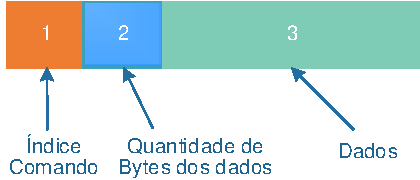
\includegraphics[width=10cm]{img8}  %pode alterar o tamanho
					\caption[Estrutura de um pacote I2C]{\label{img8}Estrutura de um pacote I2C}
				\end{center}		
			\end{figure}
			
			Como dito anteriormente, os dados que representam o estado do sistema, não correspondem a um array de bytes. Portanto, foi necessário converter as informações float e digitais para bytes para possibilitar a transmissão do mesmo. No Arduino isso foi feito utilizando a declaração union. Essa técnica permite variáveis de diferentes tipos ocupem uma mesma região de memória, o que possibilita que a estrutura de dados anteriormente criada possua a sua representação em um array de bytes, o que é necessário para transmissão via I2C. O \autoref{cod:dadosi2c} corresponde a implementação feita.
			
			Para correta interpretação dos comandos enviados pelo mestre, foi necessário mapear ações de acordo com o índice de comando criado, ou seja, definir um protocolo básico de comunicação.
			A relação entre o índice de comando e a ação correspondente é mostrada na \autoref{tbl5}. A interpretação e execução dos comandos é feita na função onReceive. Se o comando é uma solicitação de dados, o envio é realizado na função onRequest.
						
			\begin{listing}
				\begin{minted}[bgcolor=bg,breaklines=true,tabsize=2, baselinestretch=1,fontsize=\footnotesize]{cpp}
				//estrutura de dados para envio i2c
				typedef struct processData{
					float temp1;
					float temp2;
					float temp3;
					float temp4;
					float hotflow;
					float coldflow;
					float pump_speed;
					byte bstatus;
					byte chksum;
				};
				
				typedef union I2C_Send{ //compartilha a mesma área de memória
					processData data;
					byte I2C_packet[sizeof(processData)];
				};				
				\end{minted}
				\caption{Estrutura de dados do sistema}
				\label{cod:dadosi2c}
			\end{listing}
		
		\begin{table}[!htb]
			\centering
			\caption{Definição das interpretações de comando}
			\label{tbl5}
			\def\arraystretch{1.3}
			\begin{tabular}{c p{11cm}}
				\hline
				\multicolumn{1}{c}{\textbf{Índice Comando}} & \multicolumn{1}{c}{\textbf{Ação}} \\ \hline
				
				6 & Enviar dados do sistema para o mestre \\
				49 & Ligar a bomba \\ %\hline
				50 & Desligar a bomba \\ %\hline  
				51 & Ligar aquecedor \\ %\hline
				52 & Desligar o aquecedor \\ %\hline
				53 & Alterar velocidade da bomba \\ %\hline
				\hline
			\end{tabular}
		\end{table}
		
	\section{Preparação do Raspberry PI}
		\subsection{Instalação do sistema operacional}
			Conforme mencionado na \textcolor{red}{seçãoX}, o Raspberry não possui um HD interno. Portanto, é necessário instalar o sistema operacional em um microUSB, que faz o papel de HD. O Rpi suporta vários sistemas operacionais, sendo que o sistema operacional padrão é o Raspian, uma adaptação de uma distribuição Debian\footnote{\url{https://www.debian.org/intro/about}}. Foi utilizada a versão ``Raspian Stretch With Desktop'', disponível no link \url{https://www.raspberrypi.org/downloads/raspbian/}. Basicamente, deve-se extrair a imagem baixada para o microUSB. Após esse procedimento o Raspberry Pi já pode ser inicializado.
		
		\subsection{Ativação do protocolo I2C}
			O I2C não vem habilitado por padrão no sistema operacional. É necessário entrar nas configurações do Rpi e habilitá-lo. Os passos para realizar esse procedimento estão descritos por \textcite{matt2014}. Para verificar se o i2c está corretamente habilitado, deve-se abrir um terminal e digitar o comando ``sudo i2cdetect -y 1''. O resultado é exibido na \autoref{img9}.
			
			\begin{figure}[!htb]	
				%\centering
				\captionsetup{justification=centering}
				\begin{center}
					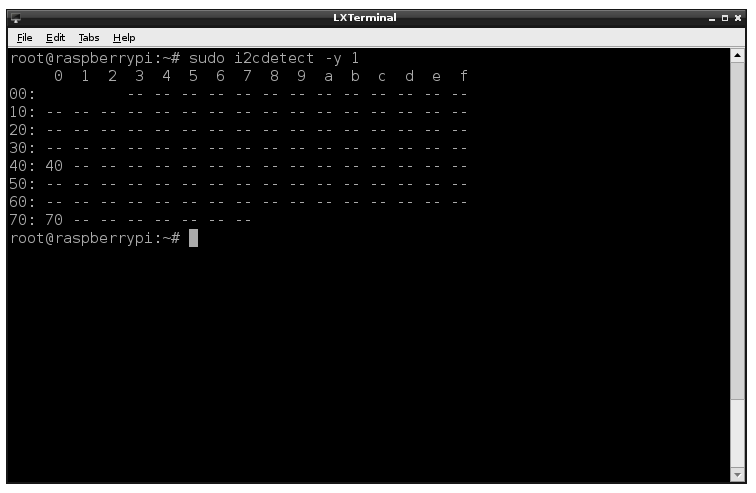
\includegraphics[width=10cm]{img9}  %pode alterar o tamanho
					\caption[I2C habilitado]{\label{img9}I2C habilitado}
				\end{center}		
			\end{figure}
		
		\subsection{Instalação de Pacotes - Python}
			O sistema operacional Raspian já possui duas versões instaladas de Python: 2.7 e 3.4. A primeira, mesmo sendo mais antiga ainda é muito utilizada pela comunidade devido à grande quantidade de pacotes desenvolvidos para essa versão; a segunda, é uma das versões mais novas disponíveis para Python.
			
			Os códigos do Gateway e do WebServer foram desenvolvidos com a versão 3.4. Antes do começo do desenvolvimento é necessário instalar os pacotes necessários para executar o projeto. Os pacotes a serem instalados dependem do propósito e característica do sistema a ser desenvolvido. É muito comum desenvolvedores trabalharem em diferentes projetos, portanto a tarefa de gerenciar os pacotes para cada projeto torna-se trabalhosa. Para isso, o Python disponibiliza a instalação de ambientes virtuais na máquina. Ambientes virtuais são diretórios para armazenar os pacotes necessários para determinados projetos. Assim, é possível isolar os arquivos de cada desenvolvimento, facilitando a mudança de um projeto para o outro \cite{kyle2017}. A utilização de ambientes virutais em Python é uma boa prática de programação e foi utilizada.
			
			Para instalar um ambiente virtual na versão python 3, é necessário utilizar os comandos descritos no \autoref{cod:venv}. Uma vez instalado, é necessário ativar o ambiente virtual. O  \autoref{cod:activate_venv} contém o código para ativá-lo. Após ativado, devem-se instalar os pacotes necessários para o projeto.  Os pacotes e as versões instaladas estão listados na \autoref{tbl6}
			
			\begin{listing}
				\begin{minted}[bgcolor=bg,breaklines=true,tabsize=2, baselinestretch=1,fontsize=\footnotesize]{bash}
				#navegar até a pasta onde se deseja instalar o ambiente virtual
				pi@raspberry $ cd pfc_env
				
				#instalar pacote virtual env
				pi@raspberry $ pip install virtualenv
				
				#criar um ambiente virtual chamado env
				pi@raspberry $ virtual env			
				\end{minted}
				\caption{Comandos para criação de um ambiente virtual}
			\label{cod:venv}
			\end{listing}
		
			\begin{listing}
				\begin{minted}[bgcolor=bg,breaklines=true,tabsize=2, baselinestretch=1,fontsize=\footnotesize]{bash}
				#ativar o diretório virtual
				pi@raspberry $ source pfc_env/bin/activate
				
				#caso o nome do diretório apareça entre parenteses como abaixo, o diretório foi ativado com sucesso
				(env) pi@raspberry $ 		
				\end{minted}
				\caption{Comandos para criação de um ambiente virtual}
				\label{cod:activate_venv}
			\end{listing}

			
			\begin{table}[!htb]
				\centering
				\caption{Pacotes necessários para o projeto}
				\label{tbl6}
				\def\arraystretch{1.3}
				\begin{tabular}{c c}
					\hline
					\multicolumn{1}{c}{\textbf{Pacote}} & \multicolumn{1}{c}{\textbf{Versão}} \\ \hline
					
					Smbus & v1.9.2 \\
					Django & v1.9.2 \\ %\hline
					Pillow & v1.9.2 \\ %\hline  
					\hline
				\end{tabular}
			\end{table}
		
			\begin{listing}
				\begin{minted}[bgcolor=bg,breaklines=true,tabsize=2, baselinestretch=1,fontsize=\footnotesize]{bash}
				#ativar o diretório virtual
				#o comando é pip install NomePacote== Versão. Exemplo:
				(env) pi@raspberry $ pip install Django==1.9.6					
				\end{minted}
				\caption{Comando para a instalação de pacotes Python}
				\label{cod:install}
			\end{listing}
		
			Todos os pacotes, com exceção do Smbus, podem ser instalados através do comando exibido no \autoref{cod:install}. É necessário ativar o ambiente virtual antes de efetuar os comandos. Para a instalação do Smbus, é necessário seguir os passos descritos por \textcite{dipto2015}. 
			
		
		
		\section{Código do Gateway}
			O código fonte completo do gateway está disponibilizado no Github, no link: \url{https://github.com/felipefonsecabh/PFC/blob/PyServeri2c/arduinoserver.py}
			
			
			
			
			


% ----------------------------------------------------------
% Resultados
% ----------------------------------------------------------
%\part{Resultados}

% ---
% primeiro capitulo de Resultados
% ---

\chapter{Resultados}



% ---
% Finaliza a parte no bookmark do PDF, para que se inicie o bookmark na raiz
% ---
\bookmarksetup{startatroot}% 
% ---

% ---
% Conclusão
% ---
\chapter[Conclusão]{Conclusão}
%\addcontentsline{toc}{chapter}{Conclusão}

\lipsum[31-33]

% ----------------------------------------------------------
% ELEMENTOS PÓS-TEXTUAIS
% ----------------------------------------------------------
\postextual


% ----------------------------------------------------------
% Referências bibliográficas
% ----------------------------------------------------------
%\bibliography{abntex2-modelo-references}
\printbibliography

% ----------------------------------------------------------
% Glossário
% ----------------------------------------------------------
%
% Consulte o manual da classe abntex2 para orientações sobre o glossário.
%
%\glossary

% ----------------------------------------------------------
% Apêndices
% ----------------------------------------------------------

% ---
% Inicia os apêndices
% ---
%\begin{apendicesenv}
%
%% Imprime uma página indicando o início dos apêndices
%\partapendices
%
%% ----------------------------------------------------------
%\chapter{Quisque libero justo}
%% ----------------------------------------------------------
%
%\lipsum[50]
%
%% ----------------------------------------------------------
%\chapter{Nullam elementum urna vel imperdiet sodales elit ipsum pharetra ligula ac pretium ante justo a nulla curabitur tristique arcu eu metus}
%% ----------------------------------------------------------
%\lipsum[55-57]
%
%\end{apendicesenv}
%% ---
%
%
%% ----------------------------------------------------------
%% Anexos
%% ----------------------------------------------------------
%
%% ---
%% Inicia os anexos
%% ---
%\begin{anexosenv}
%
%% Imprime uma página indicando o início dos anexos
%\partanexos
%
%% ---
%\chapter{Morbi ultrices rutrum lorem.}
%% ---
%\lipsum[30]
%
%% ---
%\chapter{Cras non urna sed feugiat cum sociis natoque penatibus et magnis disparturient montes nascetur ridiculus mus}
%% ---
%
%\lipsum[31]
%
%% ---
%\chapter{Fusce facilisis lacinia dui}
%% ---
%
%\lipsum[32]
%
%\end{anexosenv}
%
%%---------------------------------------------------------------------
%% INDICE REMISSIVO
%%---------------------------------------------------------------------
%
%\printindex

\end{document}
